% $HeadURL$

\chapter{Process Diagram glyphs}

%[Note on the color code: \textcolor{blue}{The glyphs that have been thorougly discussed, and are considered frozen, are represented in blue}. \textcolor{green}{The glyphs that have been thorougly discussed, but are still posing problems are represented in green}. \textcolor{red}{The glyphs that have been proposed but for which in-depth discussion is yet to come are represented in red}.]

This chapter provides a catalog of the graphical symbols available for representing entities in \PDs.  There are different classes of glyphs corresponding to different classes of material or conceptual entities, containers, processes, connecting arcs, and logical operators.  In \chap{grammar} beginning on page~\pageref{chp:grammar}, we describe the rules for combining these glyphs into a legal SBGN \PD, and in \chap{layout} beginning on page~\pageref{chp:layout}, we describe requirements and guidelines for the way that diagrams are visually organized.

\section{Overview}

% $HeadURL$

To set the stage for what follows in this chapter, we first give a brief overview of some of the concepts in the \PD notation with the help of an example shown in \fig{eg1}.

\begin{figure}[H]
  \centering
  \vspace*{-0.75em}
  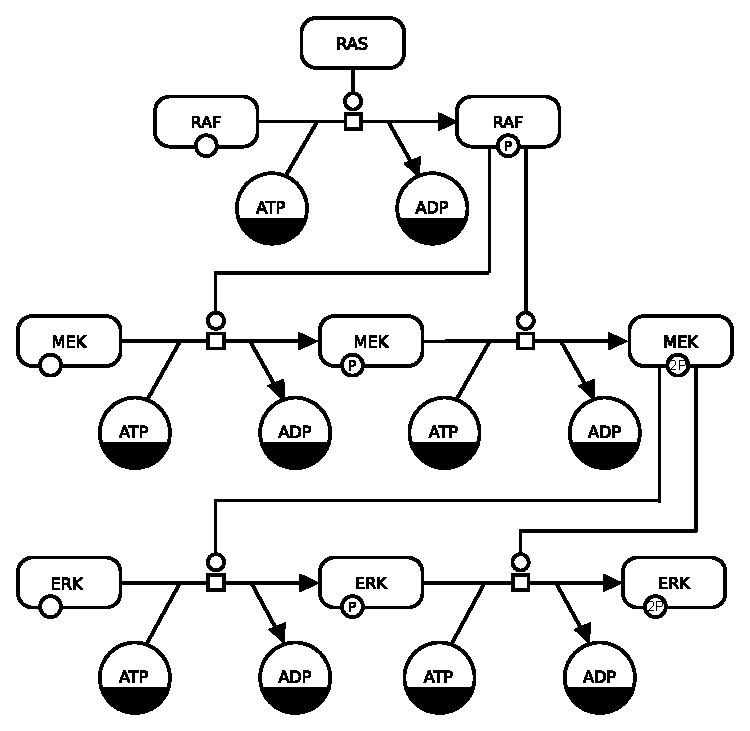
\includegraphics[scale=0.8]{examples/MAPK-only}
  \caption{This example of a \PD uses two kinds of entity pool nodes: one
    for pools of different macromolecules (\sect{macromolecule}) and
    another for pools of simple chemicals (\sect{simpleChemical}).  Most
    macromolecule nodes in this diagram are adorned with state
    variables (\sect{stateVariable}) representing phosphorylation states.
    This diagram uses one type of process node, the process node
    (\sect{process}), and one kind of connecting arc, catalysis
    (\sect{catalysis}).  Finally, some entity pool nodes have dark bands
    along their bottoms; these are clone markers indicating that the same
    pool nodes appear multiple times in the diagram.}
  \label{fig:eg1}
\end{figure}

The diagram in \fig{eg1} is a simple diagram for part of a mitogen-activated protein kinase (MAPK) cascade.  The larger nodes in the figure (some of which are in the shape of rounded rectangles and others in the shape of circles) represent biological materials---things like macromolecules and simple chemicals.  The biological materials are altered via processes, which are indicated in SBGN by lines with arrows and other decorations.  In this particular diagram, all of the processes happen to be the same: processes catalyzed by biochemical entities.  The directions of the arrows indicate the direction of the processes; for example, unphosphorylated RAF kinase processes to phosphorylated RAF kinase via a process catalyzed by RAS. Although ATP and ADP are shown as incidental to the phosphorylations on this particular graph, they are involved in the same process than the proteins getting phosphorylated. The small circles on the nodes for RAF and other entity pools represent state variables (in this case, phosphorylation sites). 

The essence of the \PD is \emph{change}: it shows how different entities in the system process from one form to another.  The entities themselves can be many different things.  In the example of \fig{eg1}, they are either pools of macromolecules or pools of simple chemicals, but as will become clear later in this chapter, they can be other conceptual and material constructs as well.  Note also that we speak of \emph{entity pools} rather than individuals; this is because in biochemical network models, one does not focus on single molecules, but rather collections of molecules of the same kind.  The molecules in a given pool are considered indistinguishable from each other.  The way in which one type of entity is transformed into another is conveyed by \emph{process nodes}, and links between entity pool nodes and process nodes indicate an influence by the entities on the processes.  In the case of \fig{eg1}, those links describe consumption \sect{consumption}, production \sect{production} and catalysis \sect{catalysis}, but others are possible.  Finally, nodes in \PDs are usually not repeated; if they do need to be repeated, they are marked with \emph{clone markers}---specific modifications to the appearance of the node (\sect{cloneMarker}). The details of this and other aspects of \PD notation are explained in the rest of this chapter.

\tab{component-summary} summarizes the different SBGN abstractions described in this chapter.

\newcolumntype{P}[1]{>{\raggedright\hspace{0pt}\arraybackslash}p{#1}}

\begin{table}[bh]
  \centering
  \small
  \begin{tabular}{@{}llP{2.4in}P{1.6in}@{}}
    \toprule
    \textbf{Component} & \textbf{Abbrev.} & \textbf{Role} & \textbf{Examples}\\
    \midrule
    Entity pool node
    & EPN
    & A population of entities that cannot be distinguished from each other
    & Specific macromolecules or other chemical species \\[0.5em]

    Container node	
    & CN
    & An encapsulation of one or more other SBGN constructs
    & Complexes, compartments \\[1.6em]

    Process node
    & PN
    & A process that transforms one or more EPNs into one or more other EPNs
    & Process, association, dissociation \\[0.5em]

    Connecting arc
    & ---
    & Links between EPNs or CNs to PNs or CNs to indicate influences
    & Production, catalysis, inhibition \\[0.5em]

    Logical operators
    & ---
    & Combines one or several inputs into one output
    & Boolean \emph{and}, \emph{or}, \emph{not} \\
    \bottomrule
  \end{tabular}
  \caption{Summary of \PD components and their roles.}
  \label{tab:component-summary}
\end{table}






%%% Local Variables: 
%%% mode: latex
%%% TeX-master: "../sbgn_PD-level1"
%%% End: 


\section{Controlled vocabularies used in \SBGNPDLone}\label{sec:CVs}

%%%%%%%%%%%%%%%%%%%%%%%%%%%%%%%%%%%%%%%%%%%%%%%%%%%%%%%%%%%%%%%%%%%%%%
%%%%                   Controlled vocabularies
%%%%%%%%%%%%%%%%%%%%%%%%%%%%%%%%%%%%%%%%%%%%%%%%%%%%%%%%%%%%%%%%%%%%%%
%\color{blue}

Some glyphs in SBGN \PDs can contain particular kinds of textual annotations conveying information relevant to the purpose of the glyph.  These annotations are \glyph{units of information} (\sect{unitInfo}) or \glyph{state variable}  (\sect{stateVariable}).  An example is in the case of multimers, which can have a unit of information conveying the number of monomers composing the multimer.  Other cases are described throughout the rest of this chapter.

The text that appears as the unit of information decorating an Entity Pool Node (EPN) must in most cases be prefixed with a controlled vocabulary term indicating the type of information being expressed.  The prefixes are mandatory except in the case of macromolecule covalent modifications (\sect{covalent-mod-cv}).  Without the use of controlled vocabulary prefixes, it would be necessary to have different glyphs to indicate different classes of information; this would lead to an explosion in the number of symbols needed.

In the rest of this section, we describe the controlled vocabularies (CVs) used in \SBGNPDLone.  They cover the following categories of information: an EPN's material type, an EPN's conceptual type, covalent modifications on macromolecules, the physical characteristics of compartments, and cardinality (\eg of multimers).  In each case, some CV terms are predefined by SBGN, but unless otherwise noted, \emph{they are not the only terms permitted}.  Authors may use other CV values not listed here, but in such cases, they should explain the terms' meanings in a figure legend or other text accompanying the diagram.


\subsection{Entity pool node material types}
\label{sec:material-types-cv}

The material type of an EPN indicates its chemical structure.  A list of common material types is shown in \tab{material-types-cv}, but others are possible.  The values are to be taken from the \sbo (\sbourl), specifically from the branch having identifier \sboid{SBO:0000240} ($\!$\emph{material entity} under \emph{participant}$\rightarrow$\emph{physical participant}).  The labels are defined by \SBGNPDLone.

\begin{table}[h]
  \centering
  \begin{tabular}{l>{\ttfamily}l>{\ttfamily}l}
    \toprule
    \textbf{Name}              & \textbf{\rmfamily Label} & \textbf{\rmfamily SBO term} \\
    \midrule
    Non-macromolecular ion     & mt:ion  & SBO:0000327\\
    Non-macromolecular radical & mt:rad  & SBO:0000328\\
    Ribonucleic acid           & mt:rna  & SBO:0000250\\
    Deoxribonucleic acid       & mt:dna  & SBO:0000251\\
    Protein                    & mt:prot & SBO:0000297\\
    Polysaccharide             & mt:psac & SBO:0000249\\
    \bottomrule
  \end{tabular}
  \caption{A sample of values from the \emph{material types} controlled
    vocabulary (\sect{material-types-cv}).}
  \label{tab:material-types-cv}
\end{table}

The material types are in contrast to the \emph{conceptual types} (see below).  The distinction is that material types are about physical composition, while conceptual types are about roles.  For example, a strand of RNA is a physical artifact, but its use as messenger RNA is a role.


\subsection{Entity pool node conceptual types}
\label{sec:conceptual-types-cv}

An EPN's \emph{conceptual type} indicates its function within the context of a given \PD.  A list of common conceptual types is shown in \tab{conceptual-types-cv}, but others are possible.  The values are to be taken from the \sbo (\sbourl), specifically from the branch having identifier \sboid{SBO:0000241} ($\!$\emph{conceptual entity} under \emph{participant}$\rightarrow$\emph{physical participant}).  The labels are defined by \SBGNPDLone.

\begin{table}[h]
  \centering
  \begin{tabular}{l>{\ttfamily}l>{\ttfamily}l}
    \toprule
    \textbf{Name}              & \textbf{\rmfamily Label} & \textbf{\rmfamily SBO term} \\
    \midrule
    Gene                      & ct:gene   & SBO:0000243\\
    Transcription start site  & ct:tss    & SBO:0000329\\
    Gene coding region        & ct:coding & SBO:0000335\\
    Gene regulatory region    & ct:grr    & SBO:0000369\\
    Messenger RNA             & ct:mRNA   & SBO:0000278\\
    \bottomrule
  \end{tabular}
  \caption{A sample of values from the \emph{conceptual types} vocabulary
    (\sect{conceptual-types-cv}).}
  \label{tab:conceptual-types-cv}
\end{table}


\subsection{Macromolecule covalent modifications}
\label{sec:covalent-mod-cv}

A common reason for the introduction of state variables (\sect{stateVariable}) on an entity is to allow access to the configuration of possible covalent modification sites on that entity.  For instance, a macromolecule may have one or more sites where a phosphate group many be attached; this change in the site's configuration (\ie being either phosphorylated or not) may factor into whether, and how, the entity can participate in different processes.  Being able to describe such modifications in a consistent fashion is the motivation for the existence of SBGN's covalent modifications controlled vocabulary.  

\tab{covalent-mod-cv} lists a number of common types of covalent modifications.  The most common values are defined by the \sbo in the branch having identifier \sboid{SBO:0000210} (\emph{addition} under \emph{events}$\rightarrow$\emph{reaction}$\rightarrow$\emph{biochemical reaction}$\rightarrow$\emph{conversion}).  The labels shown in \tab{covalent-mod-cv} are defined by \SBGNPDLone; for all other kinds of modifications not listed here, the author of a \PD must create a new label (and should also describe the meaning of the label in a legend or text accompanying the diagram).

\begin{table}[h]
  \centering
  \begin{tabular}{l>{\ttfamily}l>{\ttfamily}l}
    \toprule
    \textbf{Name}   & \textbf{\rmfamily Label} & \textbf{\rmfamily SBO term} \\
    \midrule
    Acetylation     & Ac    & SBO:0000215\\
    Glycosylation   & G     & SBO:0000217\\
    Hydroxylation   & OH    & SBO:0000233\\
    Methylation     & Me    & SBO:0000214\\
    Myristoylation  & My    & SBO:0000219\\
    Palmytoylation  & Pa    & SBO:0000218\\
    Phosphorylation & P     & SBO:0000216\\
    Prenylation     & Pr    & SBO:0000221\\
    Protonation     & H     & SBO:0000212\\
    Sulfation       & S     & SBO:0000220\\
    Ubiquitination  & Ub    & SBO:0000224\\
    \bottomrule
  \end{tabular}
  \caption{A sample of values from the \emph{covalent modifications} vocabulary
    (\sect{covalent-mod-cv}).}
  \label{tab:covalent-mod-cv}
\end{table}


\subsection{Physical characteristics of compartments}
\label{sec:physical-characteristics-cv}

\SBGNPDLone defines a special unit of information for describing certain common physical characteristics of compartments.  \tab{physical-characteristics-cv} lists the particular values defined by \SBGNPDLone.  The values correspond to the \sbo branch with identifier \sboid{SBO:0000255} (\emph{physical characteristic} under \emph{quantitative parameter}).

\begin{table}[h]
  \centering
  \begin{tabular}{l>{\ttfamily}l>{\ttfamily}l}
    \toprule
    \textbf{Name}   & \textbf{\rmfamily Label} & \textbf{\rmfamily SBO term} \\
    \midrule
    Temperature   & pc:T  & SBO:0000147\\
    Voltage       & pc:V  & SBO:0000259\\
    pH            & pc:pH & SBO:0000304\\
    \bottomrule
  \end{tabular}
  \caption{A sample of values from the \emph{physical
      characteristics} vocabulary (\sect{physical-characteristics-cv}).}
  \label{tab:physical-characteristics-cv}
\end{table}


\subsection{Cardinality}
\label{sec:cardinality-cv}

\SBGNPDLone defines a special unit of information usable on multimers for describing the number of monomers composing the multimer.  \tab{cardinality-cv} shows the way in which the values must be written.  Note that the value is a unitary number, and not (for example) a range.  There is no provision in \SBGNPDLone for specifying a range in this context because it leads to problems of entity identifiability.

\begin{table}[h]
  \centering
  \begin{tabular}{l>{\ttfamily}l>{\ttfamily}l}
    \toprule
    \textbf{Name}   & \textbf{\rmfamily Label} & \textbf{\rmfamily SBO term} \\
    \midrule
    cardinality    & N:\#  & SBO:0000364\\
    \bottomrule
  \end{tabular}
  \caption{The format of the possible values for the
    \emph{cardinality} unit of information
    (\sect{cardinality-cv}).  Here, \texttt{\#} stands for the
    number; for example, ``\texttt{N:5}''.}
  \label{tab:cardinality-cv}
\end{table}



% \normalcolor


% The following is for [X]Emacs users.  Please leave in place.
% Local Variables:
% TeX-master: "../sbgn_PD-level1"
% End:


%%%%%%%%%%%%%%%%%%%%%%%%%%%%%%%%%%%%%%%%%%%%%%%%%%%%%%%%%%%%%%%%%%%%%%
%%%%%%%%%%%%%%%%%%%%%%%%%%%%%%%%%%%%%%%%%%%%%%%%%%%%%%%%%%%%%%%%%%%%%%
%%%%                   State nodes
%%%%%%%%%%%%%%%%%%%%%%%%%%%%%%%%%%%%%%%%%%%%%%%%%%%%%%%%%%%%%%%%%%%%%%
%%%%%%%%%%%%%%%%%%%%%%%%%%%%%%%%%%%%%%%%%%%%%%%%%%%%%%%%%%%%%%%%%%%%%%

\section{Entity pool nodes}\label{sec:EPNs}

An entity pool is a population of entities that cannot be distinguished from each other, when it comes to the \SBGNPDLone map. For instance all the molecular  entities that fulfill the same role in a given process form an entity pool. As a result, an entity pool can represent different granularity levels, such as all the proteins, all the instances of a given protein, only certain forms of a given protein. To belong to a different compartment is sufficient to belong to different entity pools. Calcium ions in the endoplasmic reticulum and calcium ions in the cytosol belong to different entity pools whent it comes to representing calcium release from the endoplasmic reticulum.

\SBGNPDLone{} contains six glyphs representing classes of material entities: \glyph{unspecified entity} (\sect{unspecifiedEntity}), \glyph{simple chemical} (\sect{simpleChemical}), \glyph{macromolecule} (\sect{macromolecule}), \glyph{nucleic acid feature} (\sect{genetic}), \glyph{multimer} (\sect{multimer}) and \glyph{complex} (\sect{complex}).  (Specific types of macromolecules, such as protein, RNA, DNA, polysaccharide, and specific simple chemicals are not defined by \SBGNPDLone but may be part of future levels of SBGN.)  In addition to the material entities, \SBGNPDLone{} represents three conceptual entities: \glyph{source/sink} (\sect{sourceSink}), \glyph{perturbing agent} (\sect{perturbation}), and \glyph{tag} (\sect{tag}).  Material and conceptual entities can optionally carry auxiliary units such as \glyph{units of information} (\sect{unitInfo}), \glyph{state variables}  (\sect{stateVariable}) and \glyph{clone markers} (\sect{cloneMarker}).

% $HeadURL: https://sbgn.svn.sourceforge.net/svnroot/sbgn/trunk/documents/specifications/ProcessDiagram/Level1/sources/unspecified.tex $

\subsection{Glyph: \glyph{Unspecified entity}}
\label{sec:unspecifiedEntity}

The simplest type of EPN is the \glyph{unspecified entity}: one whose type is unknown or simply not relevant to the purposes of the model.  This arises, for example, when the existence of the entity has been inferred indirectly, or when the entity is merely a construct introduced for the needs of the model, without direct biological relevance.  These are examples of situations where the \emph{unspecified entity} glyph is appropriate.  (Conversely, for cases where the identity of the entities composing the pool \emph{is} known, there exist other, more specific glyphs described elsewhere in the \SBGNPDLone specification.)

\begin{glyphDescription}

\glyphSboTerm SBO:0000285 ! material entity of unknown nature 

\glyphContainer An \glyph{unspecified entity} is represented by an elliptic container, as shown in \fig{unspecified}.

\glyphLabel An \glyph{unspecified entity} is identified by a label placed in an unbordered box containing a string of characters.  The characters can be distributed on several lines to improve readability, although this is not mandatory.  The label box must be attached to the center of the container.  The label may spill outside of the container.

\glyphAux An \glyph{unspecified entity} may carry a \glyph{clone marker} (\sect{cloneMarker}).

\end{glyphDescription}

\begin{figure}[H]
  \centering
  \includegraphics[scale = 0.3]{images/unspecified}
  \caption{The \PD glyph for \glyph{unspecified entity}.}
  \label{fig:unspecified}
\end{figure}



% The following is for [X]Emacs users.   Please leave in place.
% Local Variables:
% TeX-master: "../sbgn_PD-level1"
% End:


\subsection{Glyph: \glyph{Simple chemical}}
\label{sec:simpleChemical}

In SBGN \PDs, a simple chemical is defined as the opposite of a macromolecule (\sect{macromolecule}): it is a chemical compound that is \emph{not} formed by the covalent linking of pseudo-identical residues.  Examples of simple chemicals are an atom, a monoatomic ion, a salt, a radical, a solid metal, a crystal, etc. A \glyph{simple chemical} is represented by a circular
container, as depicted in \fig{simpleChemical}. To avoid confusion with the Unspecified Entity (\ref{sec:unspecifiedEntity}), this glyph must remain a circle and cannot be deformed into an eclipse.

\begin{figure}[H]
  \centering
  
\includegraphics[scale = 0.3]{images/simpleChemical}
  \caption{The \PD glyph for \glyph{simple chemical}.}
  \label{fig:simpleChemical}
\end{figure}

% $HeadURL$

\paragraph{Macromolecule}
\label{sec:macromolecule}

Many biological processes involve \emph{macromolecules}: biochemical substances that are built up from the covalent linking of pseudo-identical units.  Examples of macromolecules include proteins, nucleic acids (RNA, DNA), and polysaccharides (glycogen, cellulose, starch, etc.).  Attempting to define a separate glyph for all of these different molecules would lead to an explosion of symbols in SBGN, so instead, \SBGNPDLone defines only one glyph for all macromolecules.  The same glyph is to be used for a protein, a nucleic acid, a complex sugar, and so on.  The exact nature of a particular macromolecule in a map is then clarified using its label and decorations, as will become clear below.  (Future levels of SBGN may subclass the \glyph{macromolecule} and introduce different glyphs to differentiate between types of macromolecules.)

\begin{glyphDescription}
\item[Identifying Attributes:]\mbox{}
  \begin{itemize}
  \item owning compartment
  \item name
  \item cardinality
  \item The set of state values associated with this EPN.
 \end{itemize}
\item[Special constraints or rules:]\mbox{}\newline The mutimer glyph
  must be used if cardinality is greater than 1.
\end{glyphDescription}

\subparagraph{Glyph: \glyph{Macromolecule monomer}}

This glyph represents a monomeric macromolecule.

\begin{glyphDescription}

\glyphSboTerm SBO:0000245 ! macromolecule 

\glyphContainer A macromolecule is represented by a rectangular container with rounded corners, as illustrated in \fig{macromolecule}.

\glyphLabel A \glyph{macromolecule} is identified by a label placed in an unbordered box containing a string of characters.  The characters can be distributed on several lines to improve readability, although this is not mandatory.  The label box must be attached to the center of the container.  The label may spill outside of the container.

\glyphAux A \glyph{macromolecule} can carry state variables that can add information about its state (\sect{stateVariable}).  The state of a macromolecule is therefore defined as the set of all its state variables. 

A \glyph{macromolecule} can also carry one or several \glyph{units of information} (\sect{unitInfo}).  The units of information can characterize a domain, such as a binding site.  Particular \glyph{units of information} are available for describing the material type (\sect{material-types-cv}) and the conceptual type (\sect{conceptual-types-cv}) of a macromolecule.  

\glyphCloning Labeled Clone Marker.

\end{glyphDescription}

\begin{figure}[H]
  \centering
  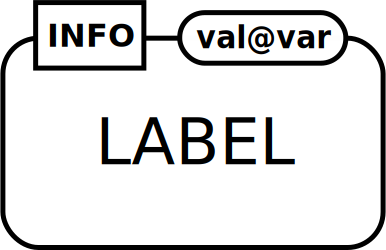
\includegraphics[width = 3in]{images/macromolecule}
  \caption{The \PD glyph for \glyph{macromolecule}, shown plain and
    unadorned on the left, and with with an additional state variable and a
    unit of information in the right and the cloned form on the right.}
  \label{fig:macromolecule}
\end{figure}


\subparagraph{Glyph: \glyph{Macromolecule multimer}}

This glyph represents a multimeric macromolecule.

\begin{glyphDescription}

\glyphSboTerm SBO:0000420 ! multimer of macromolecules

A \glyph{multimer} is represented by two identical containers shifted horizontally and vertically and stacked one on top of the other.  \fig{macromolMultimer} illustrates the glyph.

\glyphLabel As monomer

\glyphAux As monomer.

\glyphCloning Labeled Clone Marker.

\end{glyphDescription}

\begin{figure}[H]
  \centering
  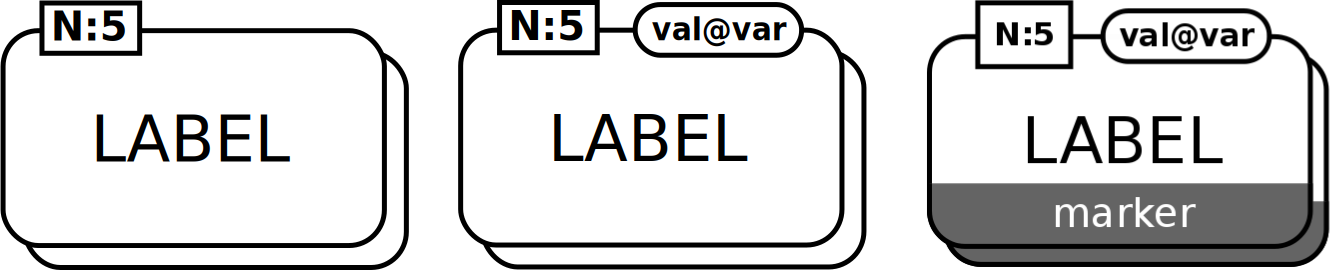
\includegraphics[width = 3.0in]{images/macromolMultimer}
  \caption{The \PD glyph for \glyph{macromolecule multimer}, shown plain and
    unadorned on the left, and with with an additional state variable and a
    unit of information on the right.}
  \label{fig:macromolMultimer}
\end{figure}




% The following is for [X]Emacs users.   Please leave in place.
% Local Variables:
% TeX-master: "../sbgn_PD-level1"
% End:

% $HeadURL$

\subsection{Glyph: \glyph{Genetic Entity}}
\label{sec:genetic}

The \emph{genetic entity} construct in SBGN is meant to represent a fragment of a macromolecule carrying genetic information.  A common use for this construct is to represent a gene or transcript.  The label of this EPN and its \emph{units of information} are often important for making the purpose clear to the reader of a diagram.

\begin{glyphDescription}

\glyphSboTerm SBO:0000354 ! genetic entity

\glyphContainer A \glyph{genetic entity} is represented by a rectangular container whose bottom half has rounded corners, as shown in \fig{genetic}.

\glyphLabel The identity of a particular \glyph{genetic entity} is established by a label placed in an unordered box containing a string of characters.  The characters may be distributed on several lines to improve readability, although this is not mandatory.  The label box must be attached to the center of the container.  The label may spill outside of the container.

\glyphAux A \glyph{genetic entity} can carry state variables (\sect{stateVariable}) that add information about its precise state.  The state of a genetic entity is therefore defined as the vector of all its state variables.  A state variable is represented by an ellipsoid container, with the long axis of the ellipsoid placed on the border of the \glyph{genetic entity}'s container as illustrated in \fig{genetic}.  The label of the state variable (type of characteristic, nucleotide number) can be optionally written either within the \glyph{genetic entity} container, or next to the border of the state variable container, or within the variable's container itself.

A \glyph{genetic information} can also carry one or several \glyph{units of information} (\sect{unitInfo}).  These can characterise a \glyph{genetic entity}'s domain, such as a binding site, or an exon.  Particular \glyph{units of information} carry the material type (\sect{material-types-cv}) and the conceptual type (\sect{conceptual-types-cv}) of the of the genetic entity.  The center of the bounding box of a \glyph{unit of information} is located on the midline of the border of the \glyph{genetic entity}.

A \glyph{genetic entity} may also carry a \glyph{clone marker}
(\sect{cloneMarker}).

\end{glyphDescription}


\begin{figure}[H]
  \centering
  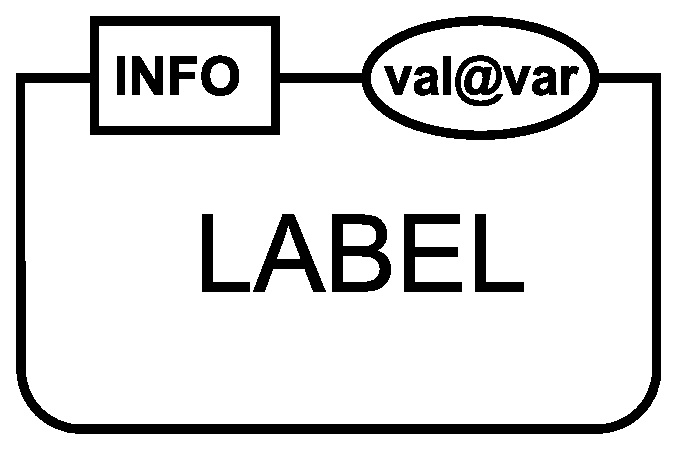
\includegraphics[scale = 0.3]{images/genetic}
  \caption{The \PD glyph for \glyph{genetic entity}.}
  \label{fig:genetic}
\end{figure}




% The following is for [X]Emacs users.  Please leave in place.
% Local Variables:
% TeX-master: "../sbgn_PD-level1"
% End:

% $HeadURL$

\subsection{Glyph: \glyph{Multimer}}
\label{sec:multimer}

As its name implies, a multimer is an aggregation of multiple identical or pseudo-identical entities held together by non-covalent bonds (Thus, they are distinguished from polymers by the fact that the later involve covalent bonds). Here,  \emph{sseudo-identical} refers to the possibility that the entities differ chemically but retain some common global characteristic, such as a structure or function, and so can be considered identical within the context of the SBGN \PD.  An example of this are the homologous subunits in a hetero-oligomeric receptor. SBGN \PD accepts multimers of \glyph{simple chemical} (\sect{simpleChemical}), \glyph{macromolecule} (\sect{macromolecule}) and \glyph{genetic entities} (\sect{genetic}).

\begin{glyphDescription}

\glyphSboTerm SBO:0000286 ! multimer

\glyphContainer A \glyph{multimer} is represented by two identical containers shifted horizontally and vertically and stacked one on top of the other.  \fig{multimer} illustrates the glyph.

\glyphLabel A \glyph{multimer} has no identity on its own.  However, the first of the monomers carries an identifying label.  The label is placed in an unbordered box containing a string of characters.  The characters can be distributed on several lines to improve readability, although this is not mandatory.  The label box must be attached to the center of the top monomer's container.  The label may spill outside of the container.

\glyphAux A \glyph{multimer} can carry state variables that can add information about its state (\sect{stateVariable}).  The state of a multimer is therefore defined as the vector of all its state variables.  Note that a \glyph{state variable} carried by a multimer actually applies to each of the constituent monomers individually.  If instead the state variables are meant to apply to the whole multimeric assembly, a \glyph{macromolecule} (\sect{macromolecule}) should be used instead of \glyph{multimer}.  An assembly containing some state variables applicable to the components, and others state variable applicable to the assembly (for instance opening of a channel and phosphorylation of each of its subunits) should be represented by a \glyph{complex} (\sect{complex}).

A \glyph{multimer} can also carry one or several \glyph{units of information} (\sect{unitInfo}).  The information can characterize a domain, such as a binding site.  Particular \glyph{units of information} exist for describing the material type (\sect{material-types-cv}), the conceptual type (\sect{conceptual-types-cv}), and the cardinality (\sect{cardinality-cv}) of the multimer.  Note that a \glyph{unit of information} carried by a multimer actually applies to each of the constituent monomers individually.  If instead a \glyph{unit of information} should be applicable to the whole multimeric assembly, a \glyph{macromolecule} should be used (\sect{macromolecule}). An assembly containing units of information applying to the components, and others to the assembly should be represented by a \glyph{complex} (\sect{complex}).

A \glyph{multimer} may also carry a \glyph{clone marker} (\sect{cloneMarker}).

\end{glyphDescription}


\begin{figure}[H]
  \centering
  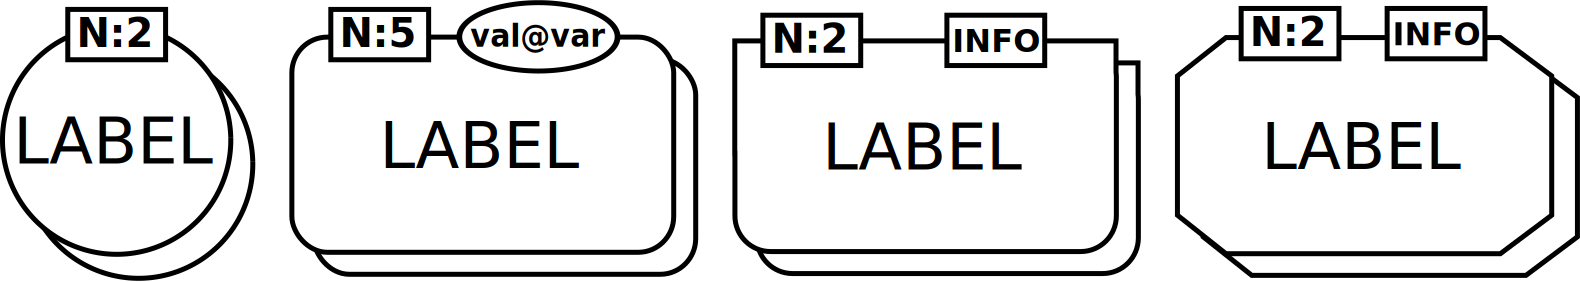
\includegraphics[scale = 0.3]{images/multimer}
  \caption{The \PD glyph for \glyph{multimer} with an additional unit of information containing the cardinality.}
  \label{fig:multimer}
\end{figure}






% The following is for [X]Emacs users.  Please leave in place.
% Local Variables:
% TeX-master: "../sbgn_PD-level1"
% End:


%%%%%%%%%%%%%%%%%%%%%%%%%%%%%%%%%%%%%%%%%%%%%%%%%%%%%%%%%%%%%%%%%%%%%%
%%%%                   Complex
%%%%%%%%%%%%%%%%%%%%%%%%%%%%%%%%%%%%%%%%%%%%%%%%%%%%%%%%%%%%%%%%%%%%%%

\subsection{Glyph: \glyph{Complex}}\label{sec:complex}

A \glyph{complex} node represents a biochemical entity composed of other biochemical entities, whether macromolecules, simple chemicals, multimers, or other complexes. The resulting entity may have its own identity, properties and function in an SBGN map. A \glyph{complex} possesses its own container box surrounding the juxtaposed container boxes of its components.  This container box is a rectangle with cut-corners (an octagonal box with sides of two different lengths).  The size of the cut-corners are adjusted so that there is no overlap between the container and the components.  The container boxes of the components must not overlap.

\begin{figure}[H]
  \centering
  \includegraphics[scale = 0.3]{images/complex}
  \caption{The \PD glyph for \glyph{complex}.}
  \label{fig:complex}
\end{figure}


Examples of \glyph{complexes} are presented in \fig{complex-examples}.

\begin{figure}[H]
  \centering
  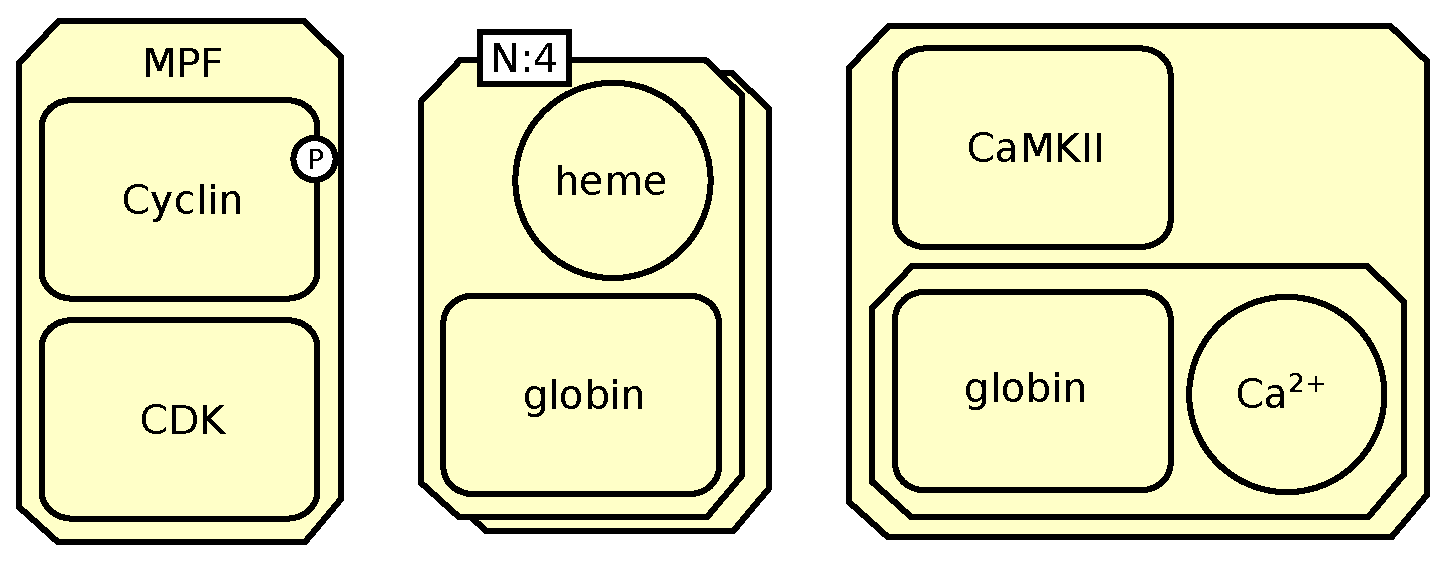
\includegraphics[scale = 0.5]{images/complex-examples}
  \caption{Examples of \glyph{complexes}. From left to right: complex between phosphorylated cyclin and CDK2 forming the maturation promoting factor in yeast, a tetramer of complexes between globin and heme, and a complex between calcium-calmodulin kinase II and another complex, itself formed of calmodulin and calcium.}
  \label{fig:complex-examples}
\end{figure}


% $HeadURL$

\subsection{Glyph: \glyph{Source/sink}}
\label{sec:sourceSink}

It is useful to have the ability to represent the creation of an entity or
a state from an unspecified source, that is, from something that one does
not need or wish to make precise.  For instance, in a model where the
production of a protein is represented, it may not be desirable to
represent all of the amino acids, sugars and other metabolites used, or the
energy involved in the protein's creation.  Similarly, we may not wish to
bother representing the details of the destruction or decomposition of some
biochemical species into a large number of more primitive entities,
preferring instead to simply say that the species ``disappears into a
sink''.  Yet another example is that one may need to represent an input
(respectively, output) into (resp. from) a compartment without explicitly
representing a transport process from a source (resp. to a target).

For these and other situations, SBGN defines a symbol for explicitly
representing the involvement of an unspecified source or sink.  The symbol
used in SBGN is borrowed from the mathematical symbol for ``empty set'',
but it is important to note that it does not actually represent a true
absence of everything or a physical void---it represents the absence of the
corresponding structures in the model, that is, the fact that these sources
or sinks are conceptualy outside the scope of the diagram.

A frequently asked question is, why bother having an explicit symbol at
all?  The reason is that one cannot simply use an arc that does not
terminate on a node, because the dangling end could be mistaken to be
pointing to another node in the diagram.  This is specially true if the
diagram is rescaled, causing the spacing of elements in the diagram to
change.  The availability and use of an explicit symbol for sources and
sinks is critical.

\begin{glyphDescription}

\glyphSboTerm SBO:0000291 ! empty set

\glyphContainer A \glyph{source/sink} is represented by a glyph for ``empty
set'', that is, a circle crossed by a bar linking the upper-right and
lower-left corners of an invisible square drawn around the circle.
\fig{sourceSink} illustrates this.  The symbol should only be linked to one
and only one edge in a diagram.

\glyphLabel An \glyph{source/sink} does not carry any labels.

\glyphAux An \glyph{source/sink} does not carry any auxiliary items.  

\end{glyphDescription}

\begin{figure}[H]
  \centering
  \includegraphics[scale = 0.3]{images/sourceSink}
  \caption{The \PD glyph for \glyph{source/sink}.}
  \label{fig:sourceSink}
\end{figure}






% The following is for [X]Emacs users.    Please leave in place.
% Local Variables:
% TeX-master: "../sbgn_PD-level1"
% End:

% $HeadURL$

\subsection{Glyph: \glyph{Perturbing agent}}
\label{sec:perturbation}
 
Biochemical networks can be affected by external influences.  Those
influences can be well-defined physical perturbations, such as a light
pulse or a change in temperature; they can also be more complex and not
well-defined phenomena, for instance a biological process, an experimental
setup, or a mutation.  For these situations, SBGN provides the
\glyph{perturbing agent} glyph. It is an EPN, and represents the amount to perturbation applied to a process.  

\begin{glyphDescription}

\glyphSboTerm SBO:0000405 ! perturbing agent

\glyphContainer A \glyph{perturbing agent} is represented by a modified hexagon
having two opposite concave faces, as illustrated in \fig{perturbation}.

\glyphLabel A \glyph{perturbing agent} is identified by a label placed in an
unbordered box containing a string of characters.  The characters can be
distributed on several lines to improve readability, although this is not
mandatory.  The label box must be attached to the center of the
\glyph{perturbing agent} container.  The label may spill outside of the container.

\glyphAux A \glyph{perturbing agent} may carry a \glyph{clone marker}
(\sect{cloneMarker}).

\end{glyphDescription}

\begin{figure}[H]
  \centering
  \includegraphics[scale = 0.3]{images/perturbation}
  \caption{The \PD glyph for \glyph{perturbing agent}.}
  \label{fig:perturbation}
\end{figure}




% The following is for [X]Emacs users.  Please leave in place.
% Local Variables:
% TeX-master: "../sbgn_PD-level1"
% End:


\subsection{Glyph: \glyph{Tag}}
\label{sec:tag}

A \glyph{tag} is a named handle, or reference, to another \glyph{EPN} (\sect{EPNs}) or \glyph{compartment} (\sect{compartment}) of the map.
Together with the \glyph{submap terminal} (\sect{submapTerminal}), it allows linking glyphs of a map to their counterpart in a submap.

\begin{glyphDescription}

\glyphSboTerm Not applicable.

\glyphIncoming
One \glyph{equivalence arc} (\sect{equivalenceArc}).

\glyphOutgoing
None.

\glyphContainer A \glyph{tag} is represented by a rectangular shape fused to an empty arrowhead, as shown in \fig{tag}.
The incoming \glyph{equivalence arc} (\sect{equivalenceArc}) must be linked to the extremity of the arrowhead.

\glyphLabel A \glyph{tag} is identified by a label that is  a string of characters that may be distributed on several lines to improve readability.
The centre of the label must be placed on the centre of the shape.
The label may extend outside of the shape.

\glyphAux 
None.

\end{glyphDescription}

\begin{figure}[H]
  \centering
  
\includegraphics{images/build/tag.pdf}
  \caption{The \PD glyph for \glyph{tag}.}
  \label{fig:tag}
\end{figure}


% $HeadURL: https://sbgn.svn.sourceforge.net/svnroot/sbgn/trunk/documents/specifications/ProcessDiagram/Level1/sources/unitInformation.tex $

\subsection{Glyph: \glyph{Unit of information}}
\label{sec:unitInfo}

When representing biological entities, it is often necessary to convey some abstract information about the entity's function that cannot (or does not need to) be easily related to its structure.  The SBGN \glyph{unit of information} is a decoration that can be used in this situation to add information to a glyph.  Some example uses include: characterizing a logical part of an entity such as a functional domain (a binding domain, a catalytic site, a promoter, etc.), or the information encoded in the entity (an exon, an open reading frame, etc.).  A \glyph{unit of information} can also convey information about the physical environment, or the specific type of biological entity it is decorating.

\begin{glyphDescription}

\glyphSboTerm Not applicable.

\glyphContainer A unit of information is represented by a rectangle.  The long side of the rectangle should be oriented parallel to the border of the \glyph{EPN} being annotated by the \glyph{unit of information}. The center of the bounding box of a \glyph{state of information} should be located on the mid-line of the border of the \glyph{EPN}.

\glyphLabel A \glyph{unit of information} is identified by a label placed in an unbordered box containing a string of characters.  The characters can be distributed on several lines to improve readability, although this is not mandatory.  The label box must be attached to the center of the container.  The label may spill outside of the container.

The label defines the information carried by the \glyph{unit of information}.  For certain predefined types of information having controlled vocabularies associated with them, SBGN defines specific prefixes that must be included in the label to indicate the type of information in question.  The controlled vocabularies predefined in \SBGNPDLone are described in \sect{CVs} and summarized in the following list:

\begin{center}
  \begin{itemize}\setlength{\parskip}{0ex}
  \item[\texttt{pc}] container physical characteristic
  \item[\texttt{mt}] entity pool material type
  \item[\texttt{ct}] entity pool conceptual type
  \item[\texttt{N}]  multimer cardinality
  \end{itemize}
\end{center}

\glyphAux A \glyph{unit of information} does not carry any auxiliary items.  

\end{glyphDescription}

\begin{figure}[H]
  \centering
  \includegraphics[scale = 0.3]{images/unitInformation}
  \caption{The \PD glyph for \glyph{unit of information}.}
  \label{fig:unitInfo}
\end{figure}




% The following is for [X]Emacs users.   Please leave in place.
% Local Variables:
% TeX-master: "../sbgn_PD-level1"
% End:



% $HeadURL$

\subsection{Glyph: \glyph{State variable}}
\label{sec:stateVariable}

Biological entities can often exist under different states that affect
their function.  These ``states'' can arise for a variety of reasons.  For
example, macromolecules can be subject to post-synthesis modifications.  In
particular, residues of macromolecules (amino acids, nucleosides, or glucid
residues) can be modified by covalent linkage to other chemicals.  Another
example of states is alternative conformations, for instance, the closed,
open or desensitized conformations of a transmembrane channel, or the
active or inactive forms of an enzyme.  When an entity can exist under
different states, the state of the whole entity (the SBGN object) can be
described by the current values of all its state variables, and the values
of the state variables of all its possible components, recursively.

\begin{glyphDescription}

\glyphSboTerm Not applicable.

\glyphContainer A state variable is represented by an ellipsoid
  container, as shown in \fig{state-var}.  The ellipsoid's long axis should
  be tangent to the border of the glyph of the EPN being modified by the
  \glyph{state variable}.

  \glyphLabel The identification of an instance of a \glyph{state variable}
  is carried by one or two unbordered boxes, each containing a string of
  characters.  The characters cannot be distributed on several lines.  One
  box is mandatory, and contains the value of the \glyph{state variable}.
  The second box is optional and carries the identification of the
  \glyph{state variable}.  This identification should be present if
  confusion is possible between several state varibles (\eg several
  phosphorylation sites).  The center of the combination of the boxes
  located in the container box is superposed to the center of this
  container box.  Optionally, the identification of the \glyph{state
    variable} can be located outside the \glyph{state variable} container
  box.  This is \textbf{strongly} discouraged.  See \fig{wrong-state-var}
  below for some examples of problems arising if the identification of a
  state variable is located outside the state variable.

\glyphAux A \glyph{state variable} does not carry any auxiliary items.  

\end{glyphDescription}

\begin{figure}[H]
  \centering
  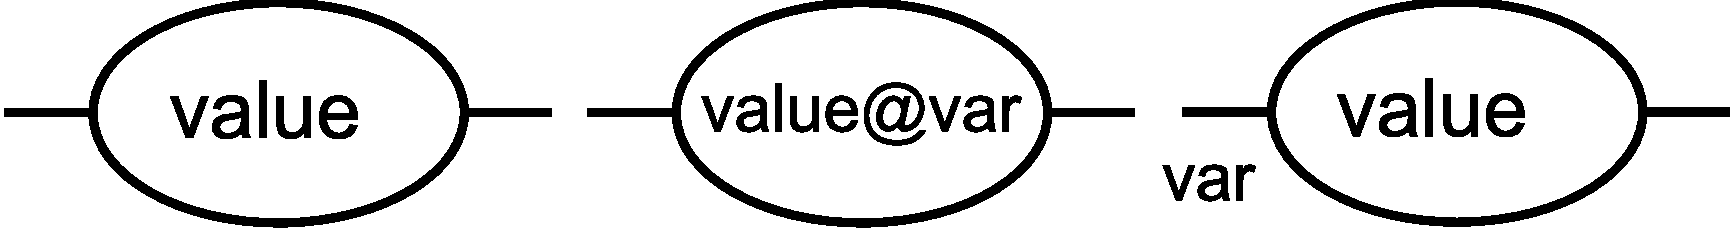
\includegraphics[scale = 0.3, trim = 0 0 0 0.25in]{images/stateVariable}
  \caption{The \PD glyph for \glyph{state variable}.}
  \label{fig:state-var}
\end{figure}

A \glyph{state variable} does not necessarily have to be a boolean-valued
variable.  For example, an ion channel can possess several conductance
states; a receptor can be inactive, active and desensitized; and so on.  A
\glyph{state variable} ``ubiquitin'' can also carry numerical values
corresponding to the number of ubiquitin molecules present in the tail.
However, a state variable can only take one defined value.  Furthermore, an
EPN's \glyph{state variable} should always be displayed and always set to a
value.  An ``empty'' \glyph{state variable} is a \glyph{state variable}
that is set to the value ``unset''.  Note that ``unset'' is \emph{not}
synonymous to ``any value'' or ``unknown value''.

The label of a state variable should, if possible, be displayed within the
ellipse.  In the top half of \fig{wrong-state-var} below, we show some
examples of pathological cases that lead to confusion in the association
between variable labels and values.  Compare the discouraged examples with
the recommended version in the bottom half of the figure.

\begin{figure}[H]
  \centering
  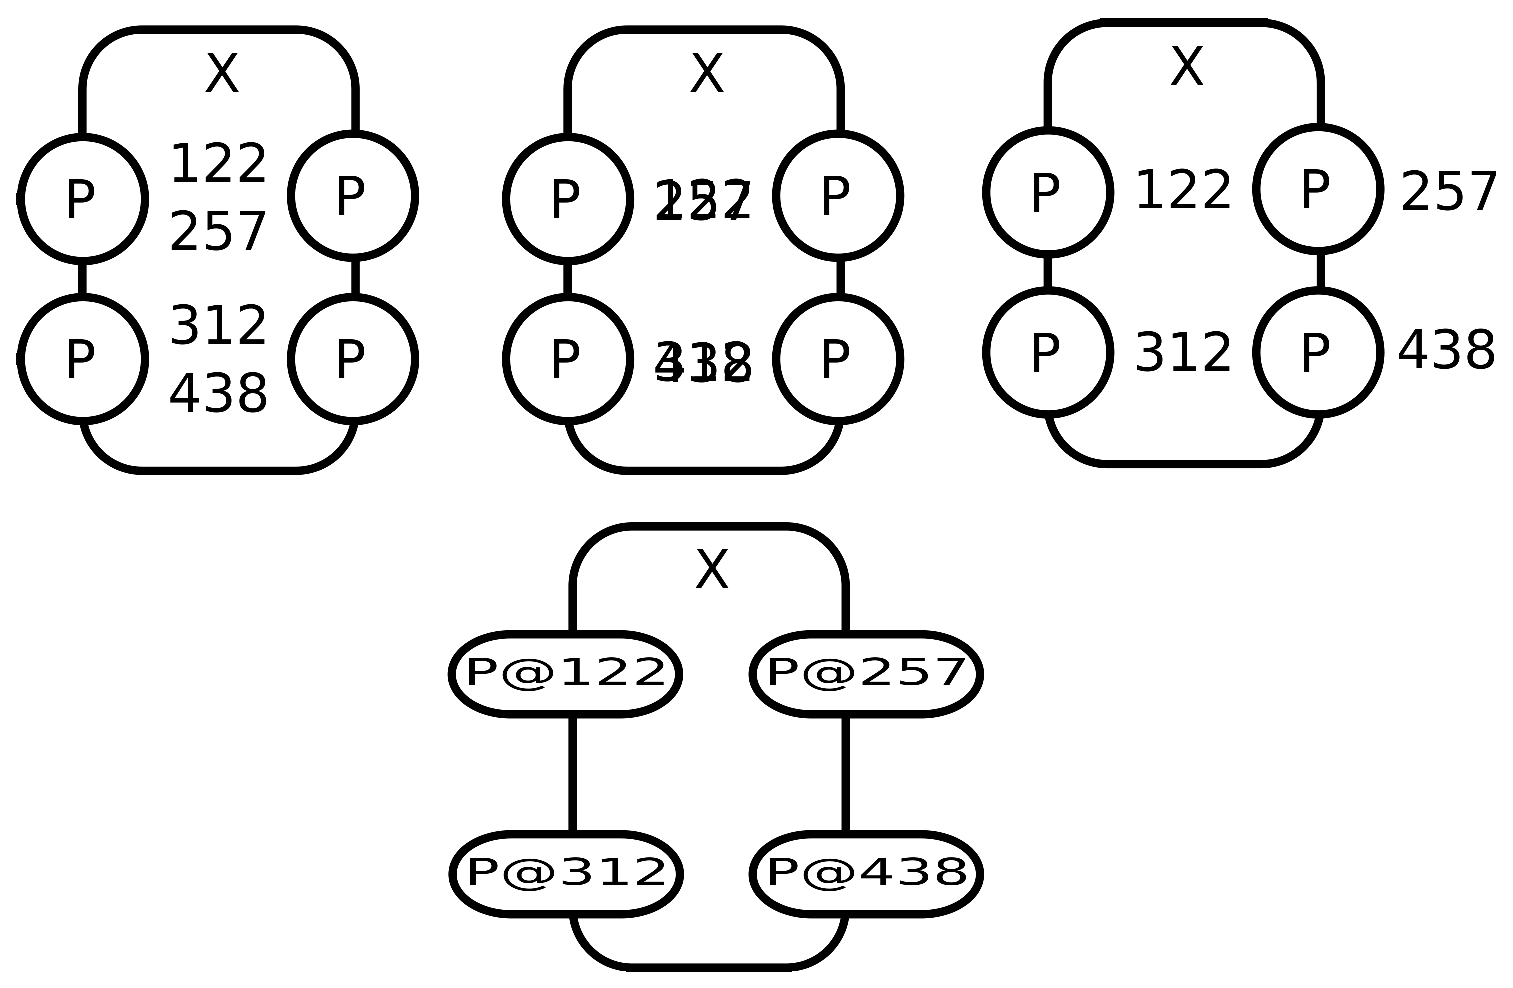
\includegraphics[scale = 0.3, trim = 0 0.5in 0 0.75in]{examples/wrongStateVariables}
  \caption{(Top) Examples of incorrect \glyph{state variables}.  (Bottom)
    Correct version.}
  \label{fig:wrong-state-var}
\end{figure}




% The following is for [X]Emacs users.  Please leave in place.
% Local Variables:
% TeX-master: "../sbgn_PD-level1"
% End:


% $HeadURL$

\subsection{Glyph: \glyph{Clone Marker}}
\label{sec:cloneMarker}

If an EPN is duplicated on a map, it is necessary to indicate this fact by using the \glyph{clone marker} auxiliary unit.  The purpose of this marker is to provide the reader with a visual indication that this node has been cloned, and that at least one other occurrence of the EPN can be found in the map (or in a submap; see \sect{submap}).  The clone marker takes two forms, simple and labeled, depending on whether the node being cloned can carry state variables (\ie whether it is a stateful EPN).


\subsubsection{Simple Clone Marker}

As mentioned above, the \glyph{simple clone marker} is the unlabeled version of the \glyph{clone marker}.  See below for the labeled version.


\begin{glyphDescription}

\glyphSboTerm Not applicable.

\glyphContainer The simple (unlabeled) \glyph{clone marker} is a portion of the surface of an EPN that has been modified visually through the use of a different shade, texture, or color.  \fig{simpleCloneMarker} illustrates this.  The \glyph{clone marker} occupies the lower part of the EPN glyph and the marker's surface must not exceed 30\% of the EPN's surface.

\glyphLabel Not applicable.

\glyphAux A \glyph{clone marker} does not carry any auxiliary items.

\end{glyphDescription}

\begin{figure}[H]
  \centering
  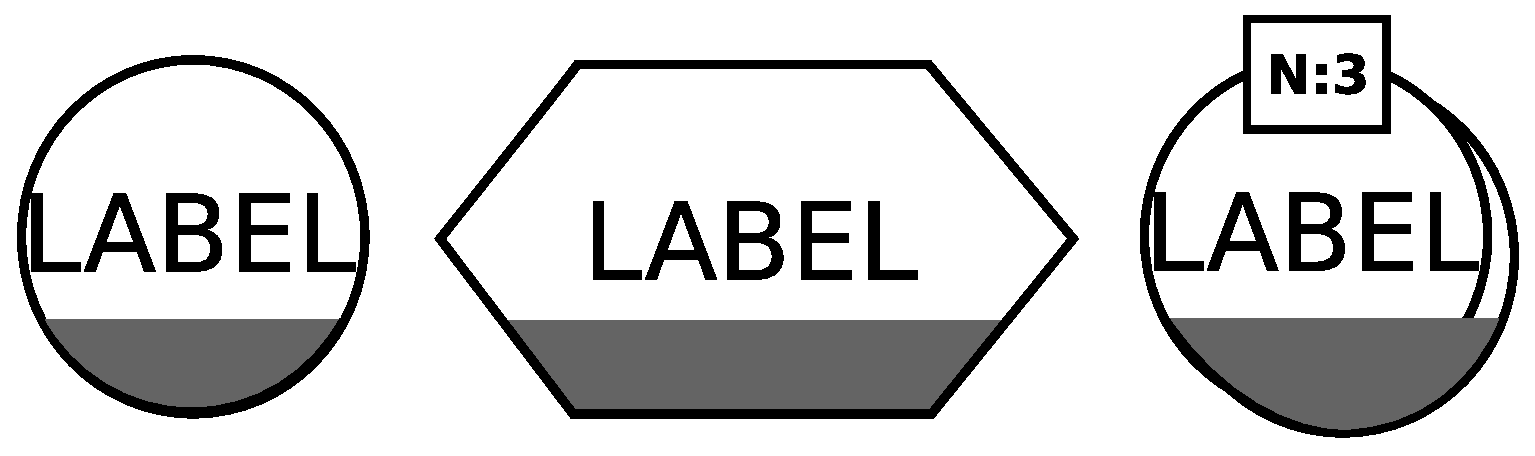
\includegraphics[scale = 0.3]{images/simpleCloneMarker}
  \caption{The \PD glyph for \glyph{clone marker}.}
  \label{fig:simpleCloneMarker}
\end{figure}


\subsubsection{Labeled Clone Marker}

Unlike the \glyph{simple clone marker}, the \glyph{labeled clone marker} includes (unsurprisingly, given its name) an identifying label that can be used to identify equivalent clones elsewhere in the diagram.  This is particularly useful for stateful EPNs, because these can have a large number of state variables displayed and therefore may be difficult to visually identify as being identical.

\begin{glyphDescription}

\glyphSboTerm Not applicable.

\glyphContainer The labeled \glyph{clone marker} is a portion of the surface of an EPN that has been modified visually through the use of a different shade, texture, or color.  The \glyph{clone marker} occupies the lower part of the EPN glyph the marker's surface must not exceed 30\% of the EPN's surface.

\glyphLabel A \glyph{clone marker} is identified by a label placed in an unbordered box containing a string of characters.  The characters can be distributed on several lines to improve readability, although this is not mandatory.  The label box must be attached to the center of the container.  The label may spill outside of the container.  The font color of the label and the color of the clone marker should contrast with one another.  The label on a labeled \glyph{labeled clone marker} is mandatory.

\glyphAux A \glyph{clone marker} does not carry any auxiliary items.

\end{glyphDescription}

\begin{figure}[H]
  \centering
  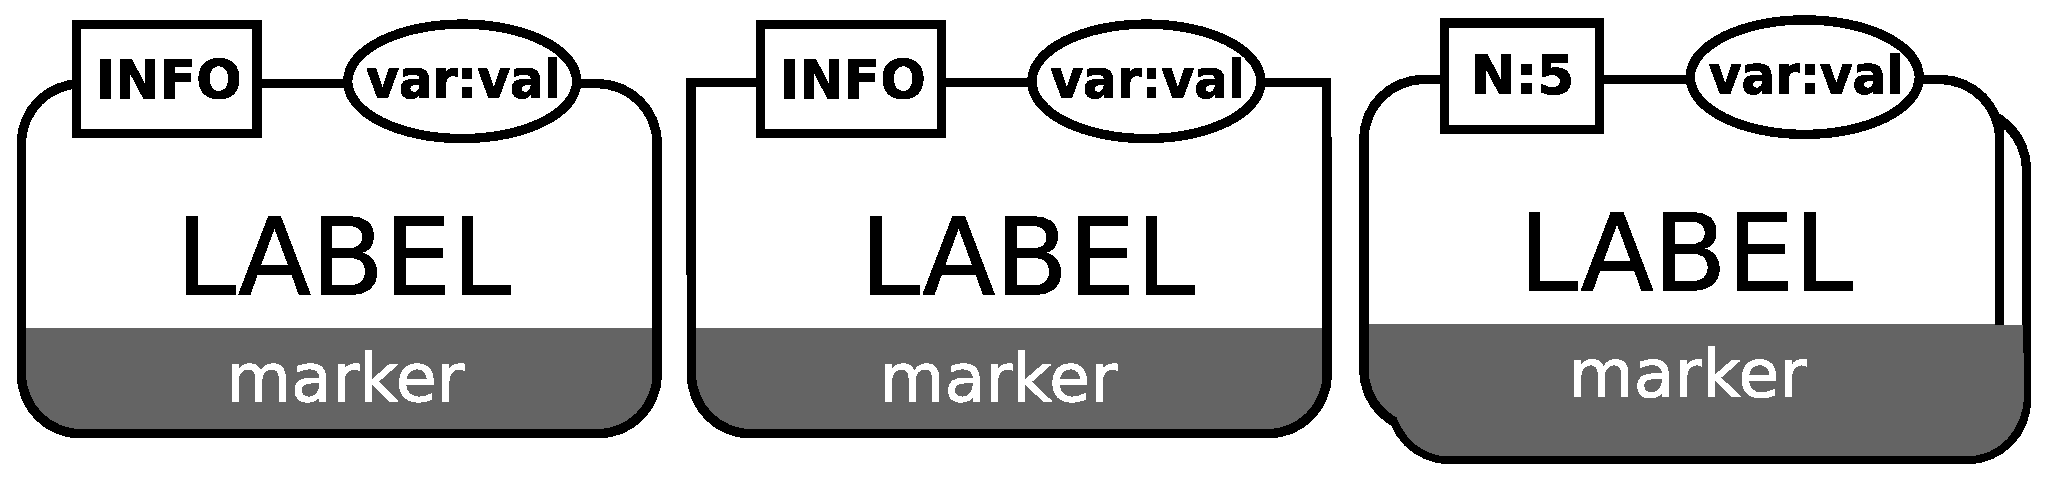
\includegraphics[scale = 0.3]{images/labeledCloneMarker}
  \caption{The \PD glyph for \glyph{labeled clone marker}.}
  \label{fig:labeledCloneMarker}
\end{figure}

\fig{example-cloning} contains an example in which we illustrate the use of \glyph{clone markers} to clone the species ATP and ADP participating in different reactions.  This example also demonstrates the chief drawbacks of using clones: it leads to a kind of dissociation of the overall network and multiplies the number of nodes required, requiring more work on the part of the reader to interpret the result.  Sometimes these disadvantages are offset in larger diagrams by a reduction in the overall number of line crossings, but not always.  In general, we advise that cloning should be used sparingly.

\begin{figure}[H]
  \centering
  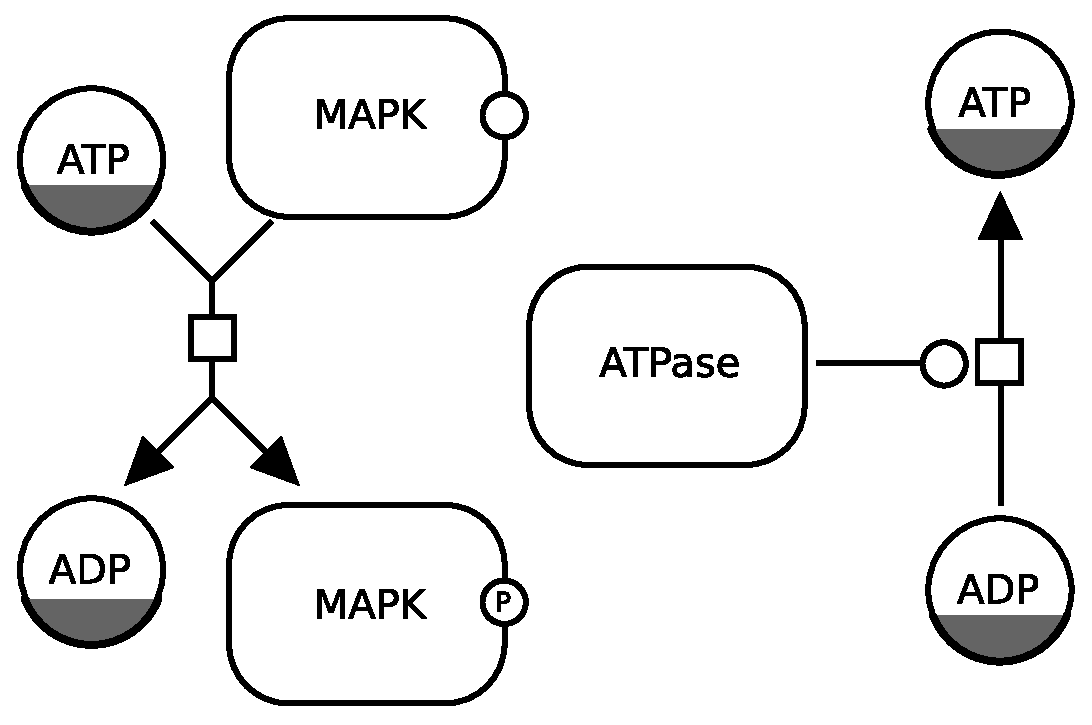
\includegraphics[scale = 0.5]{examples/cloning}
  \caption{An example of using cloning, here for the species ATP and ADP.}
  \label{fig:example-cloning}
\end{figure}




% The following is for [X]Emacs users.  Please leave in place.
% Local Variables:
% TeX-master: "../sbgn_PD-level1"
% End:


% $HeadURL$

\subsection{Examples of complex EPNs}
\label{sec:CplxEPNs}

In this section, we provide examples of Entity Pool Node representations drawn using the \SBGNPDLone glyphs described above.  The first is a representation of the calcium/calmodulin kinase II, with phosphorylation on the sites threonine 286 and 306, as well as catalytic and autoinhibitory domains.  This is shown in \fig{example-camkii}.  Note the use of \emph{units of information} and \emph{state variables}.

\begin{figure}[H]
  \centering
  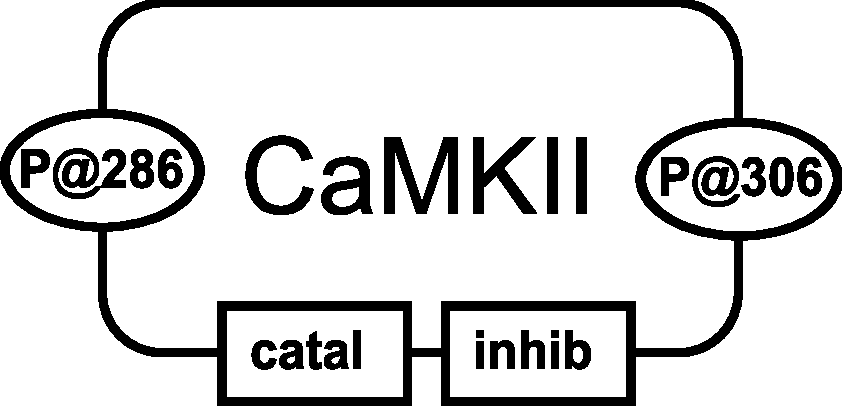
\includegraphics[scale = 0.3]{examples/macromolecule-CaMKII}
  \caption{An example representation of calcium/calmodulin kinase II.}
  \label{fig:example-camkii}
\end{figure}

The next EPN example is a representation of the glutamate receptor in the open state, with both phosphorylation and glycosylation.  The entity carries two functional domains, the ligand-binding domain and the ion pore.  \fig{example-glur} gives the diagram.

\begin{figure}[H]
  \centering
  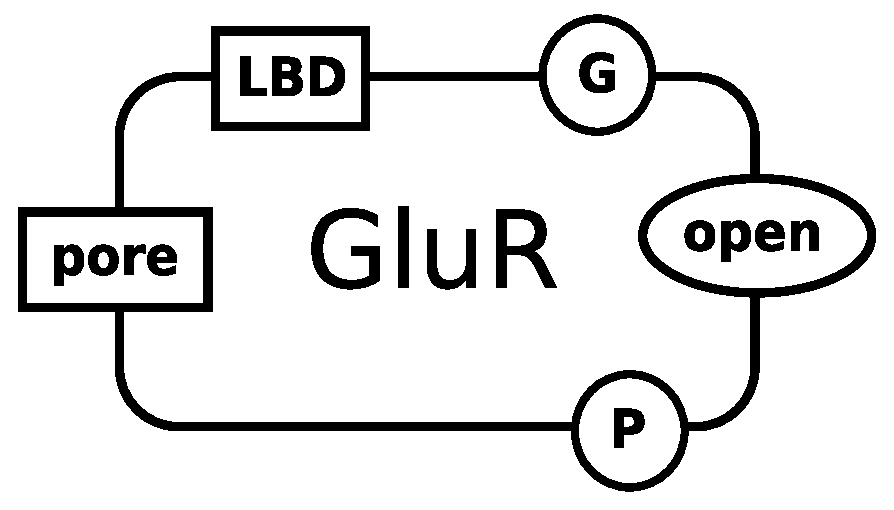
\includegraphics[scale = 0.3]{examples/macromolecule-GluR}
  \caption{An example of a glutamate receptor in the open state.}
  \label{fig:example-glur}
\end{figure}




%%% Local Variables: 
%%% mode: latex
%%% TeX-master: "../sbgn_PD-level1"
%%% End: 


%%%%%%%%%%%%%%%%%%%%%%%%%%%%%%%%%%%%%%%%%%%%%%%%%%%%%%%%%%%%%%%%%%%%%%
%%%%%%%%%%%%%%%%%%%%%%%%%%%%%%%%%%%%%%%%%%%%%%%%%%%%%%%%%%%%%%%%%%%%%%
%%%%                   Containers
%%%%%%%%%%%%%%%%%%%%%%%%%%%%%%%%%%%%%%%%%%%%%%%%%%%%%%%%%%%%%%%%%%%%%%
%%%%%%%%%%%%%%%%%%%%%%%%%%%%%%%%%%%%%%%%%%%%%%%%%%%%%%%%%%%%%%%%%%%%%%

%\section{Container nodes}\label{sec:CNs}
%%%%%%%%%%%%%%%%%%%%%%%%%%%%%%%%%%%%%%%%%%%%%%%%%%%%%%%%%%%%%%%%%%%%%%
%%%%                   Compartment
%%%%%%%%%%%%%%%%%%%%%%%%%%%%%%%%%%%%%%%%%%%%%%%%%%%%%%%%%%%%%%%%%%%%%%
%\color{blue}
\subsection{Glyph: \glyph{Compartment}}\label{sec:compartment}

In order to describe biochemical and cellular events, it is useful to
define the notion of pools. A pool is an ensemble of participants that
can be considered identical relatively to the events they are involved
into. A compartment is a logical or physical subset of the event space
that contains pools.

\begin{glyphDescription}
\glyphSboTerm  SBO:0000289 ! functional compartment 
\glyphContainer A compartment is represented by a surface
  enclosed in a continuous border or located between continuous borders. These borders should be noticeably thicker than the borders of the EPNs. A compartment can take \textbf{any} geometry. A compartment must always be entirely enclosed.
\glyphLabel The identification of the compartment is
  carried by an unbordered box containing a string of characters. The
  characters can be distributed on several lines to improve
  readability, although this is not mandatory. The label box can be
  attached anywhere in the container box. Note that the label can
  spill-over from the container box.
\glyphAux A \glyph{compartment} can carry a
  certain number of \glyph{units of information}, that will add
  information for instance about the physical environment, such as pH,
  temperature or voltage, see \ref{sec:unitInfo}.
  The center of the bounding box of a \glyph{unit of information} is
  located on the midline of the border of the compartment. 
\end{glyphDescription}

\begin{figure}[H]
  \centering
  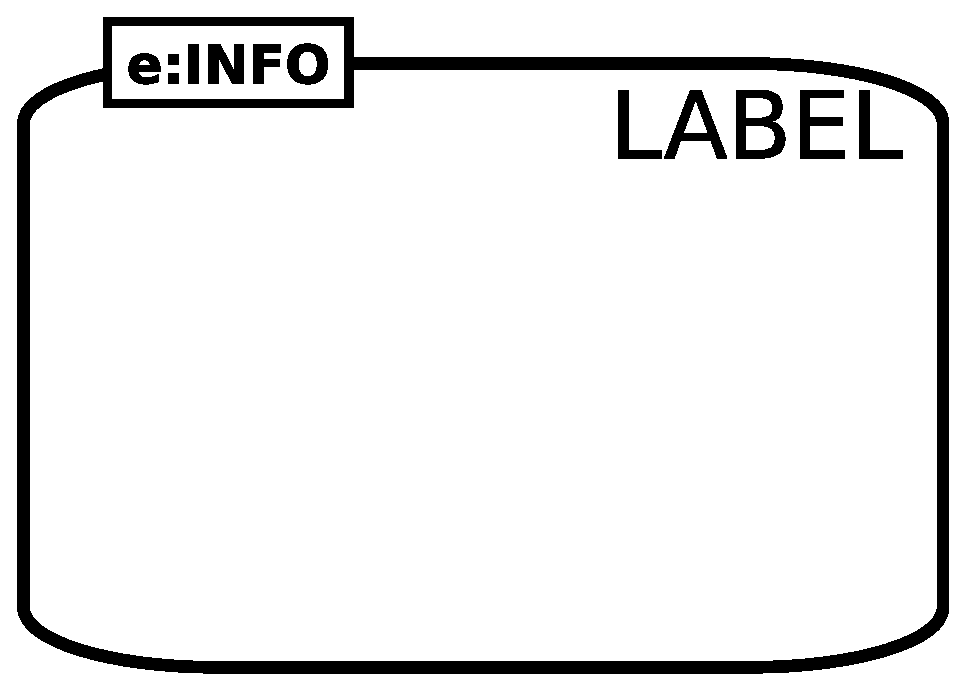
\includegraphics[scale = 0.3]{images/compartment}
  \caption{The \PD glyph for \glyph{compartment}.}
  \label{fig:compartment}
\end{figure}


It is important to note that a compartment never contains another compartment, but may surround it. Two ``adjacents'' compartments are not separated by one line, but by \textbf{two} lines. The following example represents a cell made up of a nucleus surrounded by the cytoplasm.

\begin{center}
\scalebox{0.3}{\includegraphics{examples/compartment-cell}}
\end{center}

The following example represents three adjacent compartments. Two of the compartments carry units of information. Notice the fact that those units of information do not overlap several membrane boundaries.

\begin{center}
\scalebox{0.3}{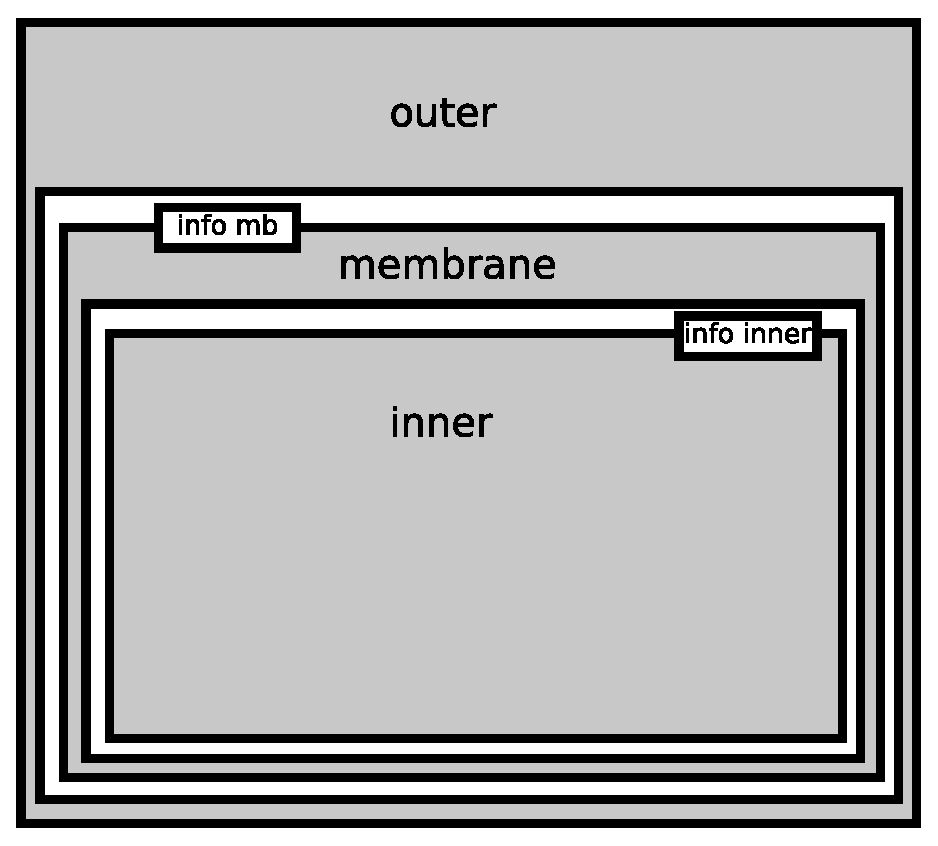
\includegraphics{examples/compartment-3comp}}
\end{center}

To make drawing aestetically more pleasing and understandable, comparments are
allowed to overlap each other visually, but it does not mean continment or
surrounding. 
The following diagram represents two equivalent
placement of compartments:

\begin{center}
\scalebox{0.3}{\includegraphics{examples/compartment_overlapping}}
\end{center}

Overlapped (hidden) part of the compartment should not contain any object,
which could be covered by overlapping compartment. The next diagram is not
correct:

\begin{center}
\scalebox{0.3}{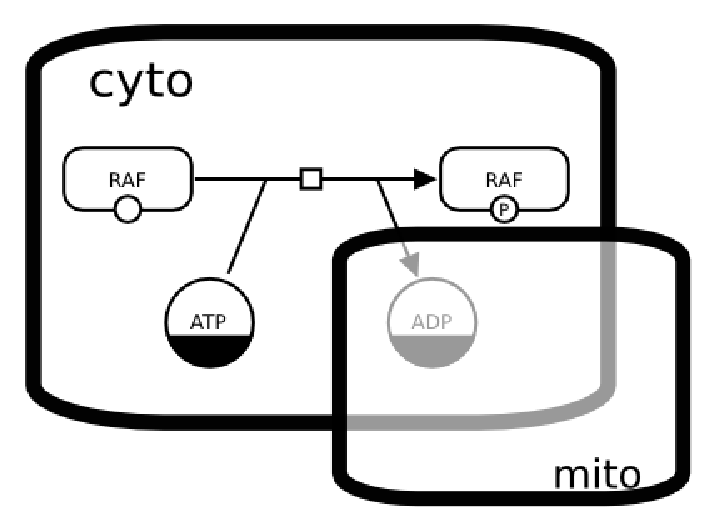
\includegraphics{examples/compartment_overlapping_wrong}}
\end{center}



%%%%%%%%%%%%%%%%%%%%%%%%%%%%%%%%%%%%%%%%%%%%%%%%%%%%%%%%%%%%%%%%%%%%%%
%%%%%%%%%%%%%%%%%%%%%%%%%%%%%%%%%%%%%%%%%%%%%%%%%%%%%%%%%%%%%%%%%%%%%%
%%%%                   Submap
%%%%%%%%%%%%%%%%%%%%%%%%%%%%%%%%%%%%%%%%%%%%%%%%%%%%%%%%%%%%%%%%%%%%%%
%%%%%%%%%%%%%%%%%%%%%%%%%%%%%%%%%%%%%%%%%%%%%%%%%%%%%%%%%%%%%%%%%%%%%%


%%%%%%%%%%%%%%%%%%%%%%%%%%%%%%%%%%%%%%%%%%%%%%%%%%%%%%%%%%%%%%%%%%%%%%
%%                     module
%%%%%%%%%%%%%%%%%%%%%%%%%%%%%%%%%%%%%%%%%%%%%%%%%%%%%%%%%%%%%%%%%%%%%%
%\color{green}
\subsection{Glyph: \glyph{Submap}}\label{sec:submap}

A \glyph{submap} is used to encapsulate a certain number of processes (including all types of nodes and edges) within one glyph. The module hides its content to the users, and display only input terminals (or ports). A module is not equivalent to an omitted process (see section~\ref{sec:omitted}). In the case of an SBGN diagram available through a software tool, the content of a module may be available to the tool. A user could then ask the tool to expand the module, for instance by clicking on the module icon, that would expand the module within the same diagram (on the same canvas) or open it in a different canvas.

\begin{glyphDescription}
\glyphSboTerm to be determined
\glyphContainer The \glyph{submap} is represented as a square box, to remind that it is fundamentaly a process.
\glyphLabel The identification of the \glyph{submap} is carried by an unbordered box containing a string of
  characters. The characters may be distributed on several lines to improve readability, although this is not mandatory.  The label box has to be attached to the center of the container box.
\glyphAux A \glyph{submap} carries labeled terminals. When the submap is represented folded, those terminals are linked to external EPNs (section~\ref{sec:EPNs}) or containers (section~\ref{sec:CNs}). In the unfolded view, exposing the internal structure of the submap, a set of \glyph{tags} point to the corresponding internal EPNs (section~\ref{sec:EPNs}) or containers (section~\ref{sec:CNs}).
\end{glyphDescription}

\begin{figure}[H]
  \centering
  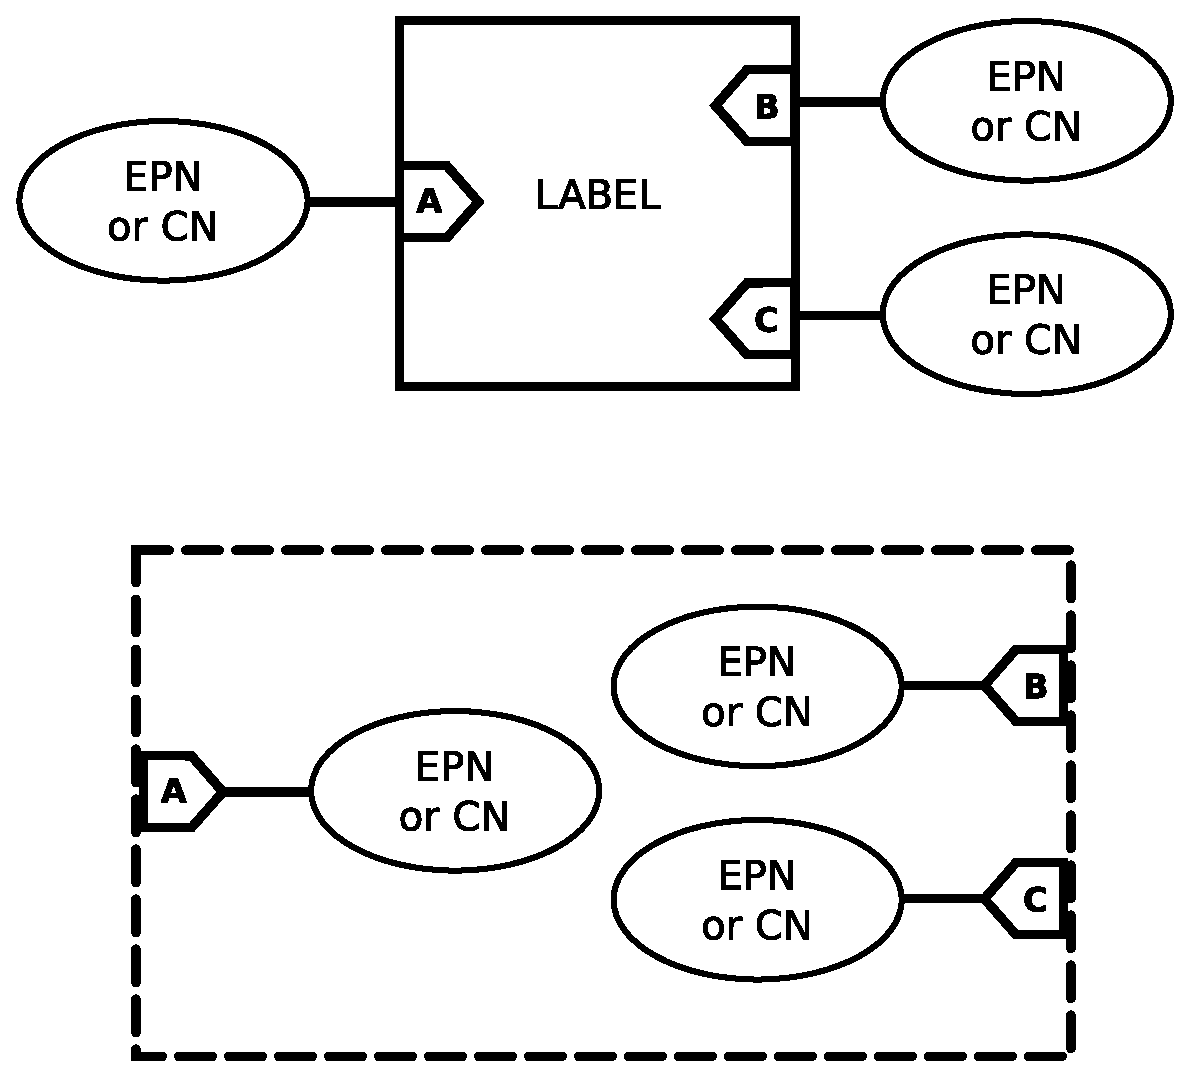
\includegraphics[scale = 0.3]{images/submap}
  \caption{The \PD glyph for \glyph{submap}.}
  \label{fig:submap}
\end{figure}


The following diagram represents a \glyph{submap} that transforms glucose into fructose-6-phosphate. The \glyph{submap} carry five terminals, four linked to EPNs and one linked to a \glyph{compartment}. The latter is particularly important in the case of EPNs present only in a \glyph{compartment} enclosed in a \glyph{submap}, and that are not linked to terminals themselves. Note that the terminals do not define a ``direction'', such as input or output. The flux of the reactions is determined by the context.

\begin{center}
\scalebox{0.3}{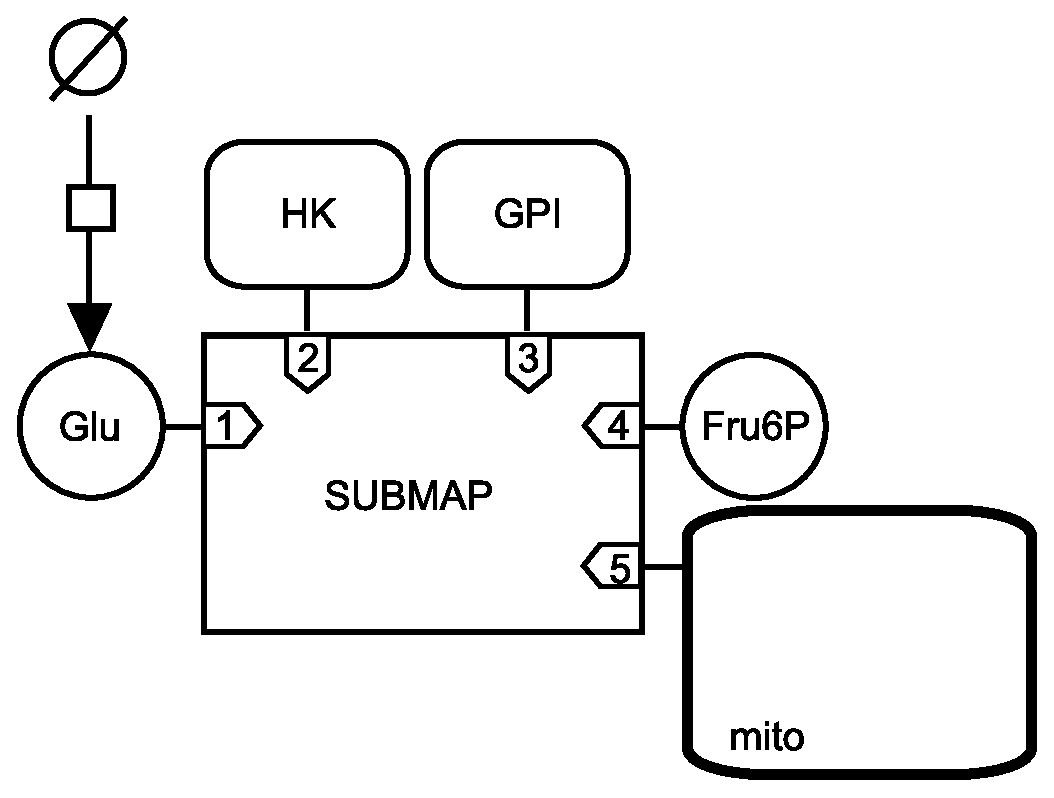
\includegraphics{examples/submap-folded}}
\end{center}

The following diagram represents an unfolded version of the submap. Here, anything outside the submap has disappeared, and the internal \glyph{tags} are not linked to the corresponding external \glyph{terminals}. Note the tag 5, linking the compartment ``mito'' of the submap to the to the compartment ``mito'' outside the submap. The compartment containing Glu6P is implicitely defined as the same than the compartment containing Glu and Fru6p. There is no ambiguity because if Glu and Fru6 were in different compartments, one of them should have been defined within the submap.

\begin{center}
\scalebox{0.3}{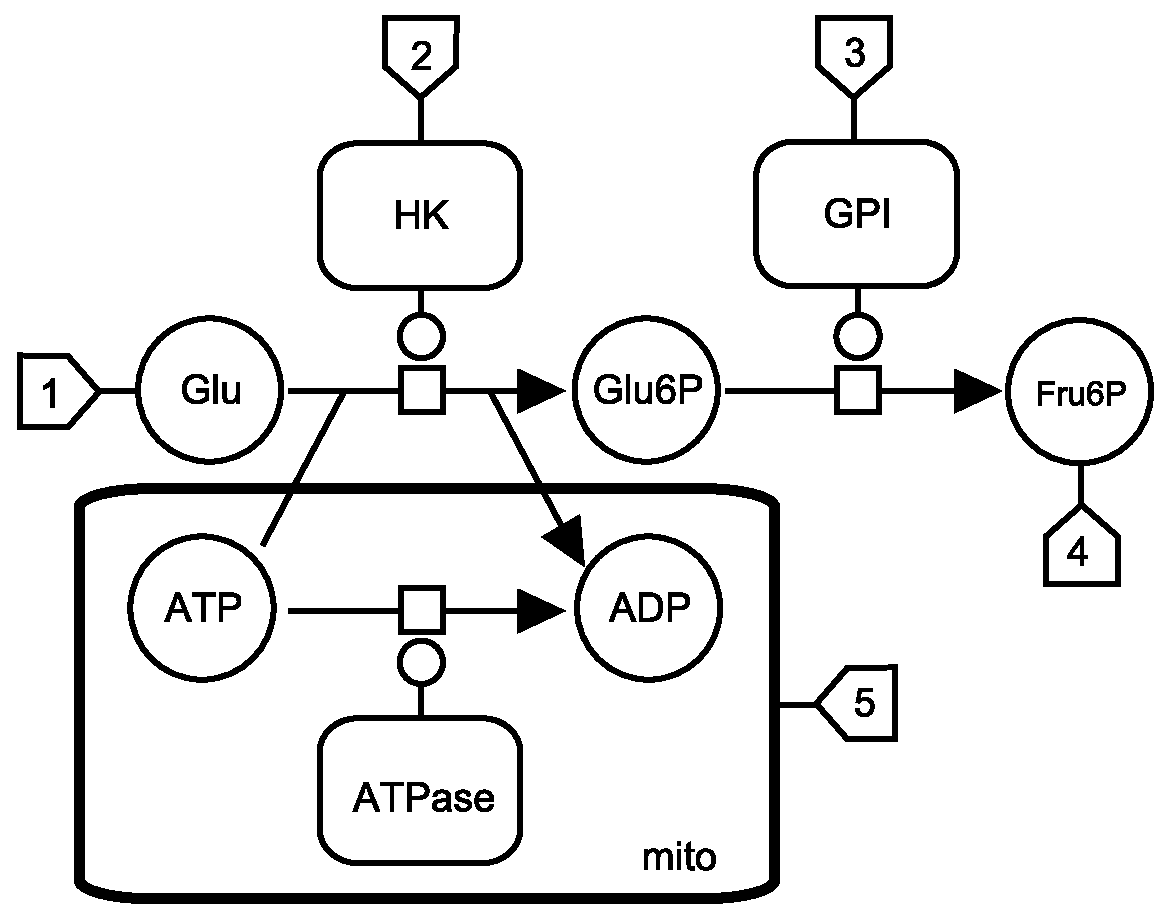
\includegraphics{examples/submap-dissociated}}
\end{center}






%%%%%%%%%%%%%%%%%%%%%%%%%%%%%%%%%%%%%%%%%%%%%%%%%%%%%%%%%%%%%%%%%%%%%%
%%%%%%%%%%%%%%%%%%%%%%%%%%%%%%%%%%%%%%%%%%%%%%%%%%%%%%%%%%%%%%%%%%%%%%
%%%%                   Process nodes
%%%%%%%%%%%%%%%%%%%%%%%%%%%%%%%%%%%%%%%%%%%%%%%%%%%%%%%%%%%%%%%%%%%%%%
%%%%%%%%%%%%%%%%%%%%%%%%%%%%%%%%%%%%%%%%%%%%%%%%%%%%%%%%%%%%%%%%%%%%%%

\section{Process nodes}\label{sec:PNs}

Process nodes represent processes that transform one or several EPNs into one or several different EPNs.   \SBGNPDLone defines a generic \glyph{process} (\sect{process}), as well as five more specific ones: the \glyph{omitted process} (\sect{omitted}), the \glyph{uncertain process} (\sect{uncertain}), the \glyph{association} (\sect{association}) and the \glyph{dissociation} (\sect{dissociation}), and the \glyph{observable} (\sect{observable}).  In future levels of the SBGN Process Diagram notation, more processes may be defined.  (One can even envision the development of a controlled vocabulary of processes, as is done now for \glyph{EPNs}; see \sect{CVs}.)

%%%%%%%%%%%%%%%%%%%%%%%%%%%%%%%%%%%%%%%%%%%%%%%%%%%%%%%%%%%%%%%%%%%%%%
%%                     Process
%%%%%%%%%%%%%%%%%%%%%%%%%%%%%%%%%%%%%%%%%%%%%%%%%%%%%%%%%%%%%%%%%%%%%%

\subsection{Glyph: \glyph{Process}}
\label{sec:process}

A process is the basic process node in SBGN.  It describes a process that transforms a given set of biochemical entities---macromolecules, simple chemicals or unspecified entities---into another set of biochemical entities.  Such a transformation might imply modification of covalent bonds (conversion), modification of the relative position of constituents (conformational process) or movement from one compartment to another (translocation). A process transforms a set of entity pools (represented by \glyph{EPNs} in \SBGNPDLone) into another set of entity pools. A \glyph{process} is represented by a square box linked to two connectors, small arcs attached to the centers of opposite sides. The consumption (\sect{consumption}) and production (\sect{production}) arcs are linked to the extremities of those connectors. The modulatory arcs (\sect{arcs}) point to the other two sides of the box. A \glyph{process} connected to \glyph{production} arcs on opposite sides is a reversible process. 

\begin{figure}[H]
  \centering
  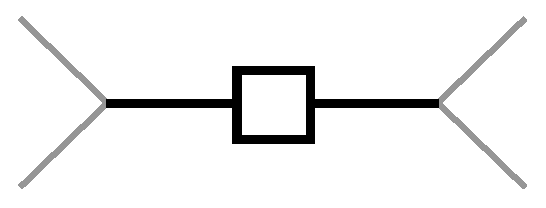
\includegraphics[scale = 0.4]{images/process}
  \caption{The \PD glyph for \glyph{process}.}
  \label{fig:process}
\end{figure}

The example in \fig{trans-react} illustrates the use of a \glyph{process} node to represent a reaction between two reactants that generates three products. The stoichiometry for each entity pool involved is 1, and therefore can be omitted.  

\begin{figure}[H]
  \centering
  \includegraphics[scale = 0.5]{images/process-reaction}
  \caption{Reaction between ATP and fructose-6-phosphate to produce fructose-1,6-biphosphate, ADP and a proton.}
  \label{fig:trans-react}
\end{figure}

The example in \fig{trans-phos} illustrates the use of a \glyph{process} node to represent the phosphorylation of a protein. 

\begin{figure}[H]
  \centering
  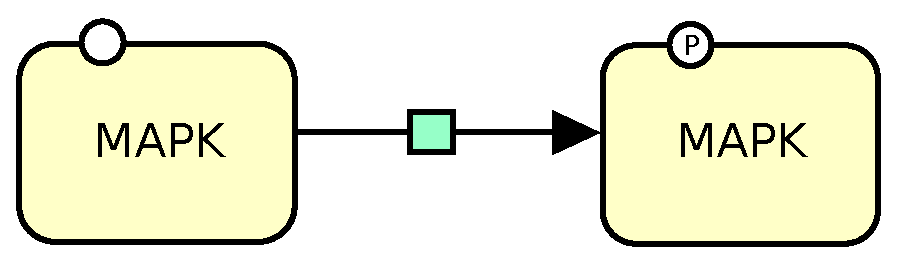
\includegraphics[scale = 0.5]{images/process-phosphorylation}
  \caption{Phosphorylation of the protein MAP kinase.}
  \label{fig:trans-phos}
\end{figure}


The example in \fig{trans-trans} illustrates the use of a \glyph{process} node to represent a translocation. The large round-cornered rectangle represents a compartment border (see \sect{compartment}).

\begin{figure}[H]
  \centering
  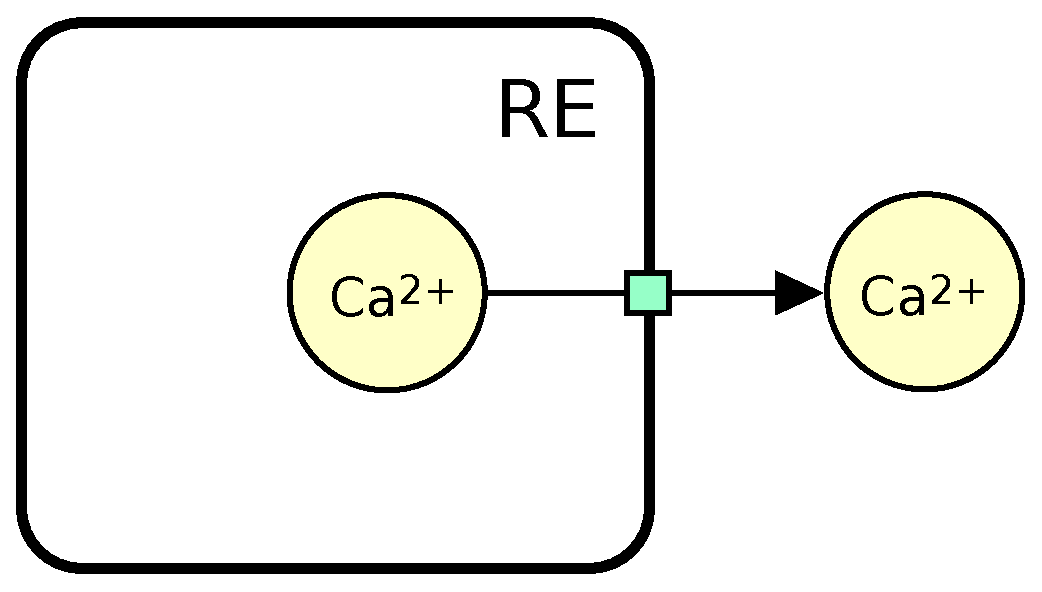
\includegraphics[scale = 0.5]{images/process-translocation}
  \caption{Translocation of calcium ion out of the endoplasmic reticulum. Note that the \glyph{process} does not have to be located on the boundary of the \glyph{compartment}. A \glyph{process} is not attached to any \glyph{compartment}.}
  \label{fig:trans-trans}
\end{figure}

The example in \fig{trans-dim} presents the conversion of two galactoses into a lactose.  Galactoses are represented by only one \glyph{simple chemical}, the cardinality being carried by the \glyph{consumption} arc.

\begin{figure}[H]
  \centering
  
\includegraphics[scale = 0.5]{images/process-dimerisation}
  \caption{Conversion of two galactoses into a lactose.}
  \label{fig:trans-dim}
\end{figure}


%%%%%%%%%%%%%%%%%%%%%%%%%%%%%%%%%%%%%%%%%%%%%%%%%%%%%%%%%%%%%%%%%%%%%%
%%                     Omitted Process
%%%%%%%%%%%%%%%%%%%%%%%%%%%%%%%%%%%%%%%%%%%%%%%%%%%%%%%%%%%%%%%%%%%%%%
%\color{blue}
\subsection{Glyph: \glyph{Omitted process}}\label{sec:omitted}

Omitted processes are processes that are known to exist, but are omitted from the diagram for the sake of clarity or parsimony. A single \glyph{omitted process} can represent any number of actual processes. The omitted process is different from a module.

\begin{glyphDescription}
 \item[SBO]\mbox{}\\ To be determined
 \item[origin]\mbox{}\\ One or several \glyph{consumption} arcs (section \ref{sec:consumption}) or one or several \glyph{production} arcs (section~\ref{sec:production}).
 \item[target]\mbox{}\\ One or several \glyph{production} arcs(section \ref{sec:production}).
 \item[node]\mbox{}\\ Omitted processes are represented as a transition containing a double slanted NW-SE line separated by an empty space.
 \end{glyphDescription}

\begin{figure}[H]
  \centering
  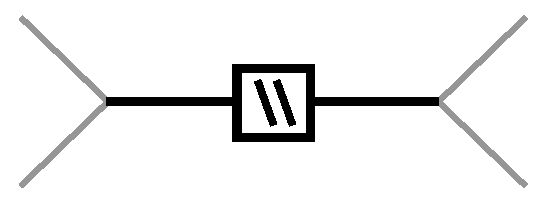
\includegraphics[scale = 0.5]{images/omitted}
  \caption{The \PD glyph for \glyph{omitted}.}
  \label{fig:omitted}
\end{figure}




%%%%%%%%%%%%%%%%%%%%%%%%%%%%%%%%%%%%%%%%%%%%%%%%%%%%%%%%%%%%%%%%%%%%%%
%%                     Uncertain Process
%%%%%%%%%%%%%%%%%%%%%%%%%%%%%%%%%%%%%%%%%%%%%%%%%%%%%%%%%%%%%%%%%%%%%%
%\color{blue}
\subsection{Glyph: \glyph{Uncertain process}}\label{sec:uncertain}

Uncertain processes are processes that may not exist. A single \glyph{uncertain process} can represent any number of actual processes. \glyph{Uncertain process} would be used to represent hypothesis, reactions which existence is supported by weak evidence etc. An \glyph{uncertain process} is represented by a \glyph{process} which square box contains a question mark.

\begin{figure}[H]
  \centering
  \includegraphics[scale = 0.5]{images/uncertain}
  \caption{The \PD glyph for an \glyph{uncertain process}.}
  \label{fig:uncertain}
\end{figure}


%%%%%%%%%%%%%%%%%%%%%%%%%%%%%%%%%%%%%%%%%%%%%%%%%%%%%%%%%%%%%%%%%%%%%%
%%                     Association
%%%%%%%%%%%%%%%%%%%%%%%%%%%%%%%%%%%%%%%%%%%%%%%%%%%%%%%%%%%%%%%%%%%%%%
%\color{blue}
\subsection{Glyph: \glyph{Association}}\label{sec:association}

The association between two EPNs represents the non-covalent binding of the biological objects represented by those EPNs into a larger complex.

\begin{glyphDescription}
 \item[SBO]\mbox{}\\ SBO:0000177 ! binding.
 \item[origin]\mbox{}\\ More than one \glyph{consumption} arcss (section \ref{sec:consumption}).
 \item[target]\mbox{}\\  One \glyph{production} arc (section \ref{sec:production}).
 \item[node]\mbox{}\\ An \glyph{association} between several entities is represented by a filled disc.
 \end{glyphDescription}

\begin{figure}[H]
  \centering
  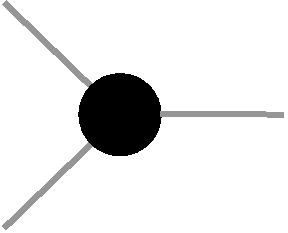
\includegraphics[scale = 0.5]{images/association}
  \caption{The \PD glyph for \glyph{association}.}
  \label{fig:association}
\end{figure}

The following example illustrates the association of two cyclin and CDC2 kinase into the Maturation Promoting Factor in ST.

\begin{center}
\scalebox{0.3}{\includegraphics{examples/association-MPF}}
\end{center}

The following example illustrates the association of a pentameric macromolecule (a nicotinic acetylcholine receptor) with a simple chemical (the local anesthetic chlorpromazin) in an unamed complex, in an ST diagram. 

\begin{center}
\scalebox{0.3}{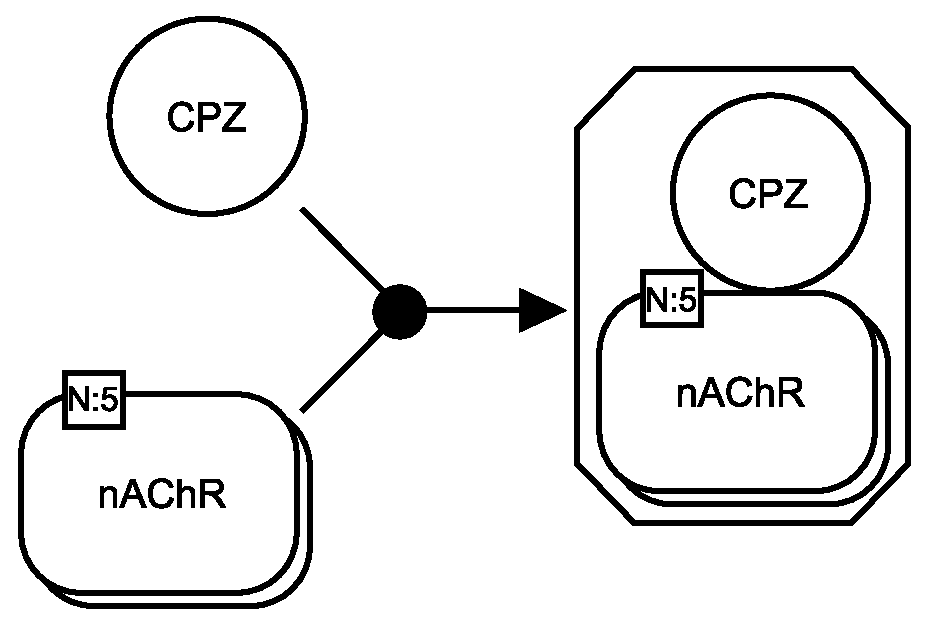
\includegraphics{examples/association-unamed}}
\end{center}

An association does not obligatory results in the formation of a \glyph{complex}, but can also produce a \glyph{multimer}. See the formation of the hemoglobin below.

\begin{center}
\scalebox{0.3}{\includegraphics{examples/association-multimerisation}}
\end{center}
\normalcolor


\subsection{Glyph: \glyph{Dissociation}}
\label{sec:dissociation}

The \glyph{dissociation} of an \glyph{EPN} into one or more \glyph{EPNs} represents the rupture of a non-covalent binding between the biological entities represented by those \glyph{EPNs}.

\begin{glyphDescription}

\glyphSboTerm
SBO:0000180 ! dissociation

\glyphIncoming
One \glyph{consumption} arc (\sect{consumption}), zero or more \glyph{modulation} arcs (\sect{modulations}).

\glyphOutgoing
One or more \glyph{production} arcs (\sect{production}).

\glyphContainer
A \glyph{process} is represented by a circular shape containing another concentric circle.
The shape is linked to two ports, that are small arcs attached to the centres of opposite sides of the shape, as shown in \fig{dissociation}.
The incoming \glyph{consumption} (\sect{consumption}) and outgoing \glyph{production} (\sect{production}) arcs are linked to the extremities of those ports.

The \glyph{modulation arcs} (\sect{modulations}) point to the other two sides of the shape.

\glyphLabel
None.

\glyphAux
None.

\end{glyphDescription}

\begin{figure}[H]
  \centering
  \includegraphics{images/build/dissociation.pdf}
  \caption{The \PD glyph for \glyph{dissociation}.}
  \label{fig:dissociation}
\end{figure}

The example in \fig{dissoc-ribo} illustrates the dissociation of the small and large ribosomal subunits from a messenger RNA.

\begin{figure}[H]
  \centering
  \includegraphics[scale = 0.8]{images/build/dissociation_ribosome_example.pdf}
  \caption{Dissociation of the small and large ribosomal subunits from a messenger RNA.}
  \label{fig:dissoc-ribo}
\end{figure}

% $HeadURL: https://sbgn.svn.sourceforge.net/svnroot/sbgn/trunk/documents/specifications/ProcessDiagram/Level1/sources/observable.tex $

\subsection{Glyph: \glyph{Observable}}
\label{sec:observable}

A biochemical network can generate phenotypes or affect biological
processes.  Such processes can take place at different levels and are
independent of the biochemical network itself.  To represent these
processes in a diagram, SBGN defines the \glyph{observable} glyph.

\begin{glyphDescription}

\glyphSboTerm SBO:0000358 ! observable

\glyphContainer An \glyph{observable} is represented by an elongated
hexagon, as illustrated in \fig{observable}.

\glyphLabel An \glyph{observable} is identified by a label placed in an
unbordered box containing a string of characters.  The characters can be
distributed on several lines to improve readability, although this is not
mandatory.  The label box must be attached to the center of the
\glyph{observable} container.  The label may spill outside of the container.

\glyphAux An \glyph{observable} may carry a \glyph{clone marker}
(\sect{cloneMarker}).

\end{glyphDescription}
 
\begin{figure}[H]
  \centering
  \includegraphics[scale = 0.3]{images/observable}
  \caption{The \PD glyph for \glyph{observable}.}
  \label{fig:observable}
\end{figure}






% The following is for [X]Emacs users.   Please leave in place.
% Local Variables:
% TeX-master: "../sbgn_PD-level1"
% End:


%%%%%%%%%%%%%%%%%%%%%%%%%%%%%%%%%%%%%%%%%%%%%%%%%%%%%%%%%%%%%%%%%%%%%%
%%%%%%%%%%%%%%%%%%%%%%%%%%%%%%%%%%%%%%%%%%%%%%%%%%%%%%%%%%%%%%%%%%%%%%
%%%%                  Arcs
%%%%%%%%%%%%%%%%%%%%%%%%%%%%%%%%%%%%%%%%%%%%%%%%%%%%%%%%%%%%%%%%%%%%%%
%%%%%%%%%%%%%%%%%%%%%%%%%%%%%%%%%%%%%%%%%%%%%%%%%%%%%%%%%%%%%%%%%%%%%%

\section{Arcs}\label{sec:arcs}

Arcs are lines that link \glyph{EPNs} and \glyph{PNs} together.  The symbols attached to their extremities indicate their semantics.

%%%%%%%%%%%%%%%%%%%%%%%%%%%%%%%%%%%%%%%%%%%%%%%%%%%%%%%%%%%%%%%%%%%%%%
%%                     Consumption
%%%%%%%%%%%%%%%%%%%%%%%%%%%%%%%%%%%%%%%%%%%%%%%%%%%%%%%%%%%%%%%%%%%%%%
%\color{blue}
\subsection{Glyph: \glyph{Consumption} }\label{sec:consumption}

\glyph{Consumption} is the arc used to represent the fact that an entity only affects a process,
but is not affected by it. 

\begin{glyphDescription}
 \item[SBO]\mbox{}\\ To be determined.
 \item[origin]\mbox{}\\ Any EPN (section \ref{sec:EPNs}).
 \item[target]\mbox{}\\ Any process node (section~\ref{sec:PNs}).
 \item[end-points]\mbox{}\\ No particular symbol is used to represent a source.
 \end{glyphDescription}


A cardinality label may be associated with \glyph{consumption} (section \ref{sec:consumption}) or 
\glyph{production} (section \ref{sec:production}) arc indicating the stoichiometry of a process. This label is a number enclosed in a rectangle with one of the long sides adjacent to the consumption arc. The cardinality is 
required to eliminate ambiguity when the exact composition, or the number of 
copies, of the inputs or outputs to a reaction are ambiguous from the diagram. 
An example is a multimer of 6 subunits dissociating into 2 monomers and 2 
dimers. Without stoichiometry labels another result, such as 4 monomers and 1 
dimer could be inferred. 
Once assigned to one arc of transition node, cardinality should be represented on
all \glyph{consumption} and \glyph{production} arcs connected to that transition
node to avoid misinterpretation.

Omitted cardinality on one edge only should not be treated as cardinality of 1, but
as unspecified cardinality. In most cases exact value could be derived from the
context, but unless cardinality is explicitly shown, it should be considered as
unspecified. In the case that stoichiometry of some part of the process is not
known, or undefined, question mark (?) should be used within cardinality label
of corresponding arcs.

\begin{figure}[H]
  \centering
  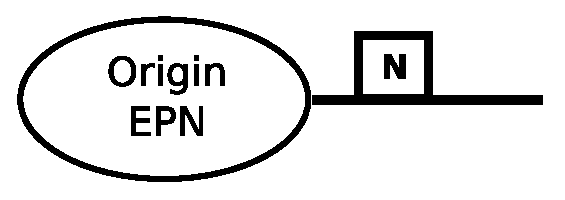
\includegraphics[scale = 0.5]{images/consumption}
  \caption{The \PD glyph for \glyph{consumption}.}
  \label{fig:consumption}
\end{figure}


%%%%%%%%%%%%%%%%%%%%%%%%%%%%%%%%%%%%%%%%%%%%%%%%%%%%%%%%%%%%%%%%%%%%%%
%%                     Production
%%%%%%%%%%%%%%%%%%%%%%%%%%%%%%%%%%%%%%%%%%%%%%%%%%%%%%%%%%%%%%%%%%%%%%

\subsection{Glyph: \glyph{Production}}\label{sec:production}

\glyph{Production} is the arc used to represent the fact that an entity pool is produced by a process. In the case of a reversible process, the 
\glyph{production} arc also acts as a \glyph{consumption} arc. The target extremity of a \glyph{production} carries a filled arrowhead. A cardinality label can be associated with a \glyph{production} arc indicating the stoichiometry of a process.

\begin{figure}[H]
  \centering
  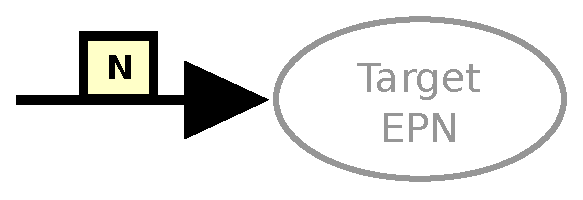
\includegraphics[scale = 0.4]{images/production}
  \caption{The \PD glyph for \glyph{production}.}
  \label{fig:production}
\end{figure}

%%%%%%%%%%%%%%%%%%%%%%%%%%%%%%%%%%%%%%%%%%%%%%%%%%%%%%%%%%%%%%%%%%%%%%
%%                     Modulation
%%%%%%%%%%%%%%%%%%%%%%%%%%%%%%%%%%%%%%%%%%%%%%%%%%%%%%%%%%%%%%%%%%%%%%
%\color{blue}
\subsection{Glyph: \glyph{Modulation}}\label{sec:modulation}

A modulation affects the flux of a process
represented by the target transition. Such a modulation can affect the
process \textbf{positively or negatively}, or even both ways depending on the
conditions, for instance the concentration of the intervening
participants. A \glyph{modulation} can also be used when one does not know the precise direction of the effect.

\begin{glyphDescription}
 \item[SBO]\mbox{}\\ SBO:0000168 ! control
 \item[origin]\mbox{}\\ Any EPN (section~\ref{sec:EPNs}) or any logical operator (section~\ref{sec:logic}).
 \item[target]\mbox{}\\ Any transition node (section~\ref{sec:PNs}).
 \item[end-points]\mbox{}\\ The target extremity of a \glyph{modulation} carries an empty diamond.
 \end{glyphDescription}

\begin{figure}[H]
  \centering
  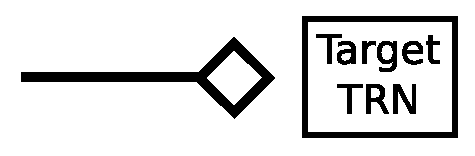
\includegraphics[scale = 0.5]{images/modulation}
  \caption{The \PD glyph for \glyph{modulation}.}
  \label{fig:modulation}
\end{figure}

The following example represents the effect of nicotine on the transition between closed and open states of nicotinic acetylcholine receptor. High concentrations of nicotine open the receptor while low concentrations can desensitize it without opening. 

\begin{center}
\scalebox{0.5}{\includegraphics{examples/modulation-nAChR}}
\end{center}

% The following example represents the effect of the voltage (a unit of information of the membrane compartment) on the opening of a sodium channel voltage-dependent. High depolarisation opens the channels while low depolarisation inactivates it (Note that the same result can be achieved with two irreversible transitions stimulated by two mutually exclusive (using \glyph{and} and \glyph{not}) units of information).
% 
% \begin{center}
% \scalebox{0.5}{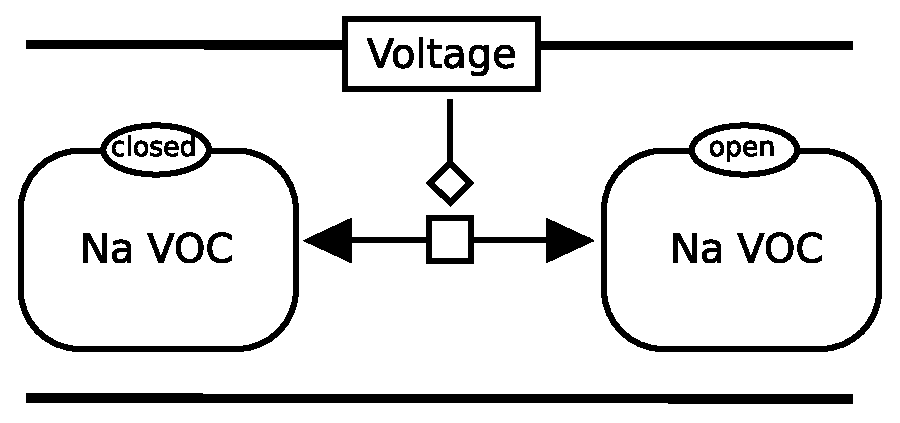
\includegraphics{examples/modulation-VOC}}
% \end{center}

\normalcolor


%%%%%%%%%%%%%%%%%%%%%%%%%%%%%%%%%%%%%%%%%%%%%%%%%%%%%%%%%%%%%%%%%%%%%%
%%                     Stimulation
%%%%%%%%%%%%%%%%%%%%%%%%%%%%%%%%%%%%%%%%%%%%%%%%%%%%%%%%%%%%%%%%%%%%%%

\subsection{Glyph: \glyph{Stimulation}}\label{sec:stimulation}
%\color{blue}

A stimulation affects \textbf{positively} the flux of a process represented by the target process. This stimulation can be for instance a catalysis or a positive allosteric regulation. Note that \glyph{catalysis} exists independently in SBGN, see \sect{catalysis}.

\begin{glyphDescription}
 \glyphSboTerm SBO:0000170 ! stimulation.
 \glyphOrigin Any \glyph{EPN} (\sect{EPNs}) or any logical operator (\sect{logic}).
 \glyphTarget Any \glyph{process node} (\sect{PNs}).
 \glyphEndPoint The target extremity of a \glyph{stimulation} carries an empty arrowhead.
 \end{glyphDescription}

\begin{figure}[H]
  \centering
  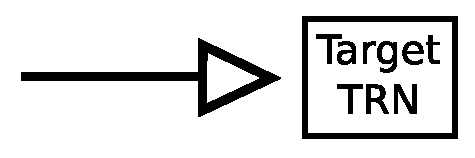
\includegraphics[scale = 0.5]{images/stimulation}
  \caption{The \PD glyph for \glyph{stimulation}.}
  \label{fig:stimulation}
\end{figure}



\subsection{Glyph: \glyph{Catalysis}}
\label{sec:catalysis}

A catalysis is a particular case of stimulation, where the effector affects positively the flux of a process represented by the target process. The positive effect on the process is due to the lowering of the activation energy of a reaction.

\begin{glyphDescription}

\glyphSboTerm
SBO:0000172 ! catalysis

\glyphOrigin
One \glyph{EPN} (\sect{EPNs}) or \glyph{logical operator} (\sect{logic}).

\glyphTarget
One \glyph{process node} (\sect{PNs}).

\glyphSymbol
The target extremity of a \glyph{catalysis} carries an empty circle, as shown in \fig{catalysis}.

\end{glyphDescription}

\begin{figure}[H]
  \centering
  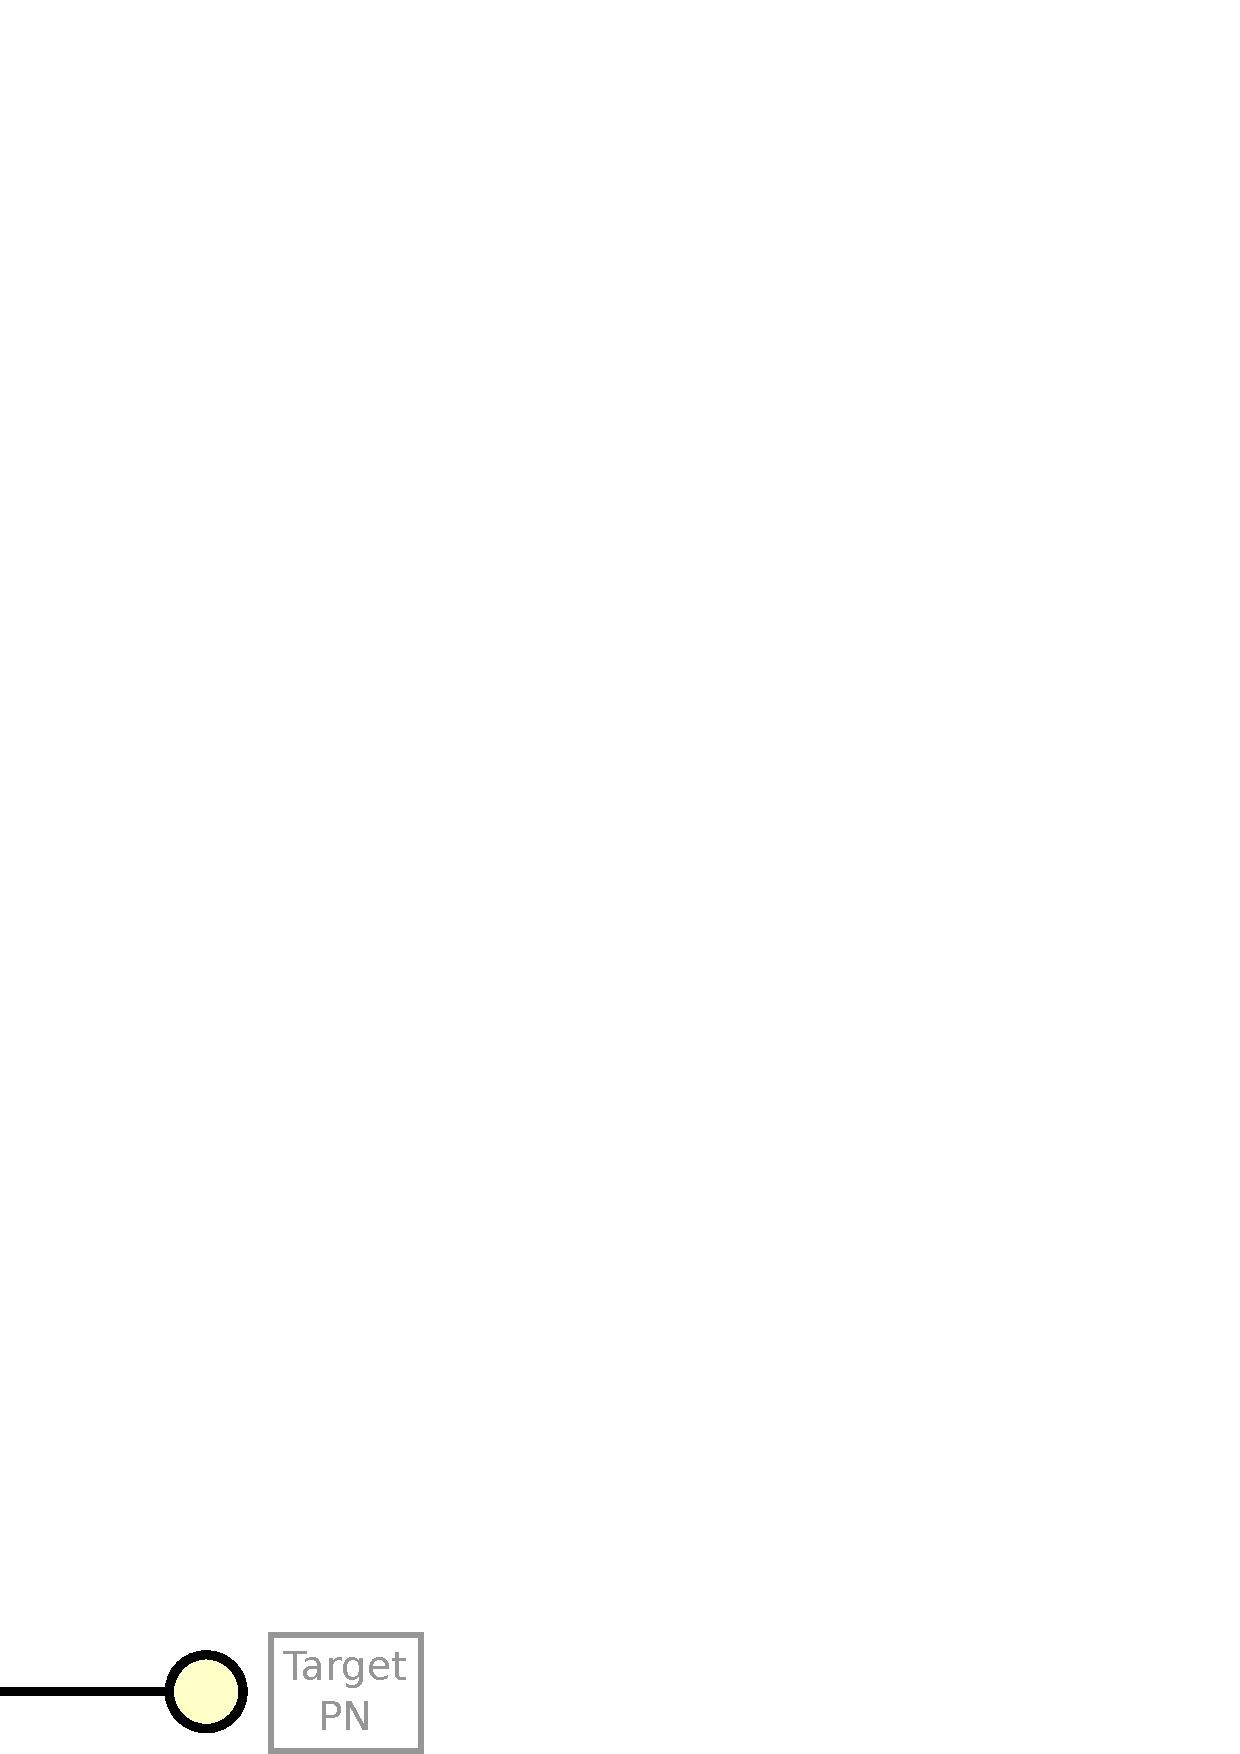
\includegraphics{images/build/catalysis.pdf}
  \caption{The \PD glyph for \glyph{catalysis}.}
  \label{fig:catalysis}
\end{figure}

%%%%%%%%%%%%%%%%%%%%%%%%%%%%%%%%%%%%%%%%%%%%%%%%%%%%%%%%%%%%%%%%%%%%%%
%%                     Inhibition
%%%%%%%%%%%%%%%%%%%%%%%%%%%%%%%%%%%%%%%%%%%%%%%%%%%%%%%%%%%%%%%%%%%%%%

\subsection{Glyph: \glyph{Inhibition}}\label{sec:inhibition}
%\color{blue}

An inhibition affects \textbf{negatively } the flux of a process represented by the target transition. This inhibition can be for instance a competitive inhibition or an allosteric inhibition. 

\begin{glyphDescription}
 \item[SBO]\mbox{}\\ SBO:0000169 ! inhibition
 \item[origin]\mbox{}\\ Any EPN (section~\ref{sec:EPNs}) or any logical operator (section~\ref{sec:logic}).
 \item[target]\mbox{}\\ Any transition node (section~\ref{sec:PNs}).
 \item[node]\mbox{}\\ The target extremity of an \glyph{inhibition} carries a bar perpendicular to the arc.
 \end{glyphDescription}

\begin{figure}[H]
  \centering
  \includegraphics[scale = 0.5]{images/inhibition}
  \caption{The \PD glyph for \glyph{inhibition}.}
  \label{fig:inhibition}
\end{figure}


\subsection{Glyph: \glyph{Necessary stimulation}}
\label{sec:necessary_stim}

A necessary stimulation is one that is necessary for a process to take place. A process modulated by a necessary stimulation can only occur when this necessary stimulation is active.

\begin{glyphDescription}

\glyphSboTerm
SBO:0000171 ! necessary stimulation

\glyphOrigin
One \glyph{EPN} (\sect{EPNs}) or 
%%%%%%%%%%%%%%%%%%%%%%%%%%%%%%%%%%%%%%%%%%%%%%%%%%%%%%%%%%%%%%%%%%%%%%
%%                     Logic arc
%%%%%%%%%%%%%%%%%%%%%%%%%%%%%%%%%%%%%%%%%%%%%%%%%%%%%%%%%%%%%%%%%%%%%%
%\color{blue}
\subsection{Glyph: \glyph{Logic arc} }\label{sec:logicArc}

\glyph{Logic arc} is used to represent the fact that an entity influences the outcome of a logic operator. A \glyph{logic arc} is represented by a simple line without particular symbols at its extremities.

\begin{figure}[H]
  \centering
  \includegraphics[scale = 0.4]{images/logicArc}
  \caption{The \PD glyph for \glyph{logic arc}.}
  \label{fig:logicArc}
\end{figure}

%%%%%%%%%%%%%%%%%%%%%%%%%%%%%%%%%%%%%%%%%%%%%%%%%%%%%%%%%%%%%%%%%%%%%%
%%                     Equivalence Arc
%%%%%%%%%%%%%%%%%%%%%%%%%%%%%%%%%%%%%%%%%%%%%%%%%%%%%%%%%%%%%%%%%%%%%%
%\color{blue}
\subsection{Glyph: \glyph{Equivalence arc} }\label{sec:equivalenceArc}

\glyph{Equivalence arc} is the arc used to represent the fact that all entities
marked by a \glyph{tag} are equivalent. An \glyph{equivalence arc} is represented by a simple line without particular symbols at its extremities.

\begin{figure}[H]
  \centering
  \includegraphics[scale = 0.4]{images/equivalence}
  \caption{The \PD glyph for \glyph{Equivalence arc}.}
  \label{fig:equivalence}
\end{figure}



%%%%%%%%%%%%%%%%%%%%%%%%%%%%%%%%%%%%%%%%%%%%%%%%%%%%%%%%%%%%%%%%%%%%%%
%%%%%%%%%%%%%%%%%%%%%%%%%%%%%%%%%%%%%%%%%%%%%%%%%%%%%%%%%%%%%%%%%%%%%%
%%%%                   Logical operators
%%%%%%%%%%%%%%%%%%%%%%%%%%%%%%%%%%%%%%%%%%%%%%%%%%%%%%%%%%%%%%%%%%%%%%
%%%%%%%%%%%%%%%%%%%%%%%%%%%%%%%%%%%%%%%%%%%%%%%%%%%%%%%%%%%%%%%%%%%%%%

\section{Logical operators}\label{sec:logic}

%%%%%%%%%%%%%%%%%%%%%%%%%%%%%%%%%%%%%%%%%%%%%%%%%%%%%%%%%%%%%%%%%%%%%%
%%                     And
%%%%%%%%%%%%%%%%%%%%%%%%%%%%%%%%%%%%%%%%%%%%%%%%%%%%%%%%%%%%%%%%%%%%%%
%\color{blue}
\subsection{Glyph: \glyph{And}}\label{sec:and}

The glyph \glyph{and} is used to denote that all the \glyph{EPNs} linked as input are necessary to produce the output.  

\begin{glyphDescription}
 \glyphSboTerm SBO:0000173 ! and.
 \glyphOrigin More than one EPN (section~\ref{sec:EPNs}) or logical operator (section~\ref{sec:logic}).
 \glyphTarget  One modulation (section~\ref{sec:modulation}), stimulation (section~\ref{sec:stimulation}), catalysis (section~\ref{sec:catalysis}), inhibition (section~\ref{sec:inhibition}) or necessary stimulation (section~\ref{sec:necessary_stim}) arc.
 \glyphNode \glyph{And} is represented by a circle carrying the word ``AND''.
\end{glyphDescription}

\begin{figure}[H]
  \centering
  \includegraphics[scale = 0.5]{images/and}
  \caption{The \PD glyph for \glyph{and}. Only two inputs are represented, but more would be allowed.}
  \label{fig:and}
\end{figure}


% The following maps illustrate the dephosphorylation of the MAP inase ERK by the protein phosphatase 2A and the STriatal Enriched Phosphatase, in ST (left) and ER (right). 
% 
% \begin{center}
% \scalebox{0.5}{\includegraphics{images/stimulation-example1}}
% \end{center}
\normalcolor

%%%%%%%%%%%%%%%%%%%%%%%%%%%%%%%%%%%%%%%%%%%%%%%%%%%%%%%%%%%%%%%%%%%%%%
%%                     Or
%%%%%%%%%%%%%%%%%%%%%%%%%%%%%%%%%%%%%%%%%%%%%%%%%%%%%%%%%%%%%%%%%%%%%%
%\color{blue}
\subsection{Glyph: \glyph{Or}}\label{sec:or}

\begin{glyphDescription}
 \glyphSboTerm SBO:0000174 ! or.
 \glyphOrigin More than one EPN (section~\ref{sec:EPNs}) or logical operator (section~\ref{sec:logic}).
 \glyphTarget  One modulation (section~\ref{sec:modulation}), stimulation (section~\ref{sec:stimulation}), catalysis (section~\ref{sec:catalysis}), inhibition (section~\ref{sec:inhibition}) or trigger (section~\ref{sec:trigger}) arc.
 \glyphNode \glyph{Or} is represented by a circle carrying the word ``OR''.
 \end{glyphDescription}

\begin{figure}[H]
  \centering
  \includegraphics[scale = 0.5]{images/or}
  \caption{The \PD glyph for \glyph{or}. Only two inputs are represented, but more would be allowed.}
  \label{fig:or}
\end{figure}



%%%%%%%%%%%%%%%%%%%%%%%%%%%%%%%%%%%%%%%%%%%%%%%%%%%%%%%%%%%%%%%%%%%%%%
%%                     Not
%%%%%%%%%%%%%%%%%%%%%%%%%%%%%%%%%%%%%%%%%%%%%%%%%%%%%%%%%%%%%%%%%%%%%%
%\color{blue}
\subsection{Glyph: \glyph{Not}}\label{sec:not}

\begin{description}
 \item[SBO]\mbox{}\\ SBO:0000238 ! not.
 \item[origin]\mbox{}\\ One EPN (section~\ref{sec:EPNs}) or logical operator (section~\ref{sec:logic}).
 \item[target]\mbox{}\\  One modulation (section~\ref{sec:modulation}), stimulation (section~\ref{sec:stimulation}), catalysis (section~\ref{sec:catalysis}), inhibition (section~\ref{sec:inhibition}) or trigger (section~\ref{sec:trigger}) arcs.
 \item[node]\mbox{}\\ \glyph{not} is represented by a circle carrying the word ``not''.
 \end{description}

\begin{figure}[H]
  \centering
  \includegraphics[scale = 0.5]{images/not}
  \caption{The \PD glyph for \glyph{not}.}
  \label{fig:not}
\end{figure}



% The following is for [X]Emacs users.  Please leave in place.
% Local Variables:
% TeX-master: "../sbgn_PD-level1"
% End:
